\documentclass[12pt , a4paper]{article}

\usepackage[french]{babel}
\usepackage [utf8] {inputenc} % utf-8 / latin1
\usepackage[T1]{fontenc}
\usepackage{aeguill} %impression de qualite des listings
\usepackage {amsmath}
\usepackage {mathpazo}
\usepackage {hyperref} %lien dynamique
\usepackage {graphicx}%image
\usepackage {fancyhdr}%entete et pied de page
\usepackage {float} %image
\usepackage {color}
\usepackage{lastpage}
\usepackage[top=2cm, bottom=2cm, left=2cm , right=2cm]{geometry}
\usepackage{vmargin}
\usepackage{listings}
\usepackage{lscape}


\definecolor{hellgelb}{rgb}{1,1,0.8}
\definecolor{colKeys}{rgb}{0,0,1}
\definecolor{colIdentifier}{rgb}{0,0,0}
\definecolor{colComments}{rgb}{0,0.5,0}
\definecolor{colString}{rgb}{0.62,0.12,0.94}

\newcommand {\TitreCours}{Java distribué}
\newcommand {\Epoque}{GM4 - 2ème semestre}
\newcommand {\Prof}{M. Pécuchet}
\newcommand {\Auteur}{Pauline Réquéna \and Guillaume Dubuisson Duplessis}

\newcommand{\J}{
  \lstset{
    language=java,
    float=hbp,
    basicstyle=\ttfamily\small,
    identifierstyle=\color{colIdentifier},
    keywordstyle=\bf \color{colKeys},
    stringstyle=\color{colString},
    commentstyle=\color{colComments},
    columns=flexible,
    tabsize=5,
    frame=single,
    % frame=shadowbox,
    rulesepcolor=\color[gray]{0.5},
    extendedchars=true,
    showspaces=false,
    showstringspaces=false,
    numbers=left,
    stepnumber=5,
    firstnumber=1,
    numberstyle=\tiny,
    breaklines=true,
    % backgroundcolor=\color{hellgelb},
    captionpos=b,%
  }
}


\title{Java distribué\\
  \vspace{0.6cm}
  \normalsize{Gestionnaire d'agendas} 
  \begin{center}
    % \includegraphics[scale=3.5]{./images/piton3d.jpg}
  \end{center}
}
\author{\Auteur}
\date{\today}

% UNE METHODE DE DEFINITION D'ENTETE
% \pagestyle{fancy}
% \fancyhf{}%detruit les entetes deja presents
% \renewcommand{\headrulewidth}{0.4pt}
% \renewcommand{\footrulewidth}{0.4pt}
% \lhead{\Auteur}
% \rhead{\today}
% \rfoot{\thepage\ sur \pageref{LastPage}}

% MEMO
% \lhead{haut gauche}
% \chead{centre haut}
% \rhead{haut droit}
% \lfoot{bas gauche}

% UNE AUTRE METHODE
% \pagestyle{headings}
\setmarginsrb{2.5cm}{1cm}{1cm}{1.5cm}{.5cm}{.5cm}{.5cm}{.5cm}
% \renewcommand{\sectionmark}[1]{\markright{\textsc{\TitreCours:} \thesection. \#1 \hrulefill\ \textup{page }}}
% FONCTIONNEMENT DE \setmarginsrb
% \setmarginsrb{1}{2}{3}{4}{5}{6}{7}{8}
% 1 est la marge gauche
% 2 est la marge en haut
% 3 est la marge droite
% 4 est la marge en bas
% 5 fixe la hauteur de l'entête
% 6 fixe la distance entre l'entête et le texte
% 7 fixe la hauteur du pied de page
% 8 fixe la distance entre le texte et le pied de page

% UNE DERNIERE METHODE
\pagestyle{fancy}
\fancyhf{}%supprime les entetes et pieds de page utilise par defaut par LaTeX
% \rightmark : contient le nom de la section courante
% \markright : contient le nom de la section courante
% \renewcommand{\sectionmark}[1]{\markright{\#1}}
% \renewcommand{\chaptermark}[1]{\markboth{\bsc{\chaptername~\thechapter{} :} #1}{}}
\renewcommand{\sectionmark}[1]{\markright{\thesection{} #1}}
\lhead[\thepage]{\TitreCours\ - \rightmark} 
\rhead{\Epoque}
\rfoot{\thepage\ / \pageref{LastPage}}

\fancypagestyle{plain}{ 
  \fancyhead{} 
  \renewcommand{\headrulewidth}{0pt}
}

\begin{document}
\maketitle
\thispagestyle{empty}
% \setcounter{page}{0}
\newpage
\thispagestyle{plain}% page sans entete 

\tableofcontents
\newpage
\section{Introduction}
\noindent A faire

\newpage
\section{Analyse détaillée du sujet}

\subsection{Description du sujet}
Le sujet de notre mini-projet de Java Distribu\'e consiste en la
conception et l{\textquoteright}impl\'ementation d{\textquoteright}un
site web de gestion d{\textquoteright}agendas. Ce site a pour fonction
de g\'erer les diff\'erents types d{\textquoteright}agendas
d{\textquoteright}un utilisateur. Par exemple, un utilisateur peut
disposer d{\textquoteright}un agenda
{\guillemotleft}~Travail~{\guillemotright} pour ses rendez-vous
professionnels et d{\textquoteright}un agenda
{\guillemotleft}~Perso~{\guillemotright} pour ses activit\'es
personnelles. Cette application permettra donc la gestion individuelle
de ces 2 agendas.


\vspace{0.5cm}

\noindent Un utilisateur de ce gestionnaire devra donc pouvoir~avoir acc\`es aux
fonctionnalit\'es suivantes :


\begin{itemize}
\item \textbf{Consulter ses agendas sous une forme claire et
    fonctionnelle}
\end{itemize}
Nous avons opt\'e pour l{\textquoteright}affichage des agendas par
semaine. Par ailleurs, afin de pouvoir bien distinguer les diff\'erents
agendas lors de l{\textquoteright}affichage des \'ev\`enements, chaque
agenda est caract\'eris\'e par une couleur.

\vspace{0.5cm}
\begin{itemize}
\item \textbf{Cr\'eer un nouvel agenda}
\end{itemize}
Un agenda est caract\'eris\'e par un nom, un lieu
d{\textquoteright}application, une description, ainsi
qu{\textquoteright}une couleur.

\vspace{0.5cm}
\begin{itemize}
\item \textbf{Modifier les param\`etres d{\textquoteright}un agenda
    pr\'eexistant}
\end{itemize}
Une fois qu{\textquoteright}un agenda a \'et\'e cr\'ee,
l{\textquoteright}utilisateur doit pouvoir s{\textquoteright}il le
souhaite en modifier les d\'etails ou la couleur
d{\textquoteright}affichage.

\vspace{0.5cm}
\begin{itemize}
\item \textbf{Supprimer un agenda pr\'eexistant}
\end{itemize}
Lorsqu{\textquoteright}un agenda n{\textquoteright}est plus utilis\'e
par l{\textquoteright}internaute, celui-ci peut le supprimer, afin de
ne pas encombrer son compte de donn\'ees inutiles. Ce
n{\textquoteright}est pas une action anodine, car toute suppression est
irr\'eversible et entra\^ine la suppression de tous \'ev\`enements de
l{\textquoteright}agenda.

\vspace{0.5cm}
\begin{itemize}
\item \textbf{Cr\'eer un nouvel \'ev\`enement dans un agenda
    pr\'eexistant}
\end{itemize}
Un \'ev\`enement appartient \`a un agenda. Il est caract\'eris\'e par un
objet, une date, un lieu, des heures de d\'ebut et de fin, ainsi
qu{\textquoteright}une description.

\vspace{0.5cm}
\begin{itemize}
\item \textbf{Modifier les caract\'eristiques d{\textquoteright}un
    \'ev\`enement pr\'eexistant}
\end{itemize}
Une fois qu{\textquoteright}un \'ev\`enement a \'et\'e cr\'ee dans un
agenda, l{\textquoteright}utilisateur doit pouvoir s{\textquoteright}il
le souhaite en modifier les d\'etails.

\vspace{0.5cm}
\begin{itemize}
\item \textbf{Supprimer un \'ev\`enement pr\'eexistant}
\end{itemize}





\newpage
\subsection{Structure du site}


L{\textquoteright}acc\`es \`a ce site se fera par le biais
d{\textquoteright}une page d{\textquoteright}authentification. En
effet, les comptes de chaque utilisateur sont confidentiels. Pour se
connecter au gestionnaire d{\textquoteright}agendas,
l{\textquoteright}internaute devra donc en premier lieu saisir son
login et son mot de passe.

\vspace{0.5cm}

\noindent Une fois l{\textquoteright}authentification accomplie,
l{\textquoteright}internaute sera dirig\'e vers la page
d{\textquoteright}accueil, compos\'ee de plusieurs parties :


\begin{itemize}
\item \textbf{L{\textquoteright}en-t\^ete}
\end{itemize}
Elle est constitu\'ee du logo de l{\textquoteright}application,
d{\textquoteright}un message d{\textquoteright}accueil et du bouton de
d\'econnexion.

\vspace{0.5cm}
\begin{itemize}
\item \textbf{Le menu de gauche~}
\end{itemize}
Ce menu est compos\'e tout d{\textquoteright}abord de la liste des
agendas de l{\textquoteright}utilisateur connect\'e. Ce dernier peut
s\'electionner dans cette liste les agendas qu{\textquoteright}il
d\'esire ou non afficher.

\noindent A travers ce menu, l{\textquoteright}utilisateur peut \'egalement
acc\'eder aux diff\'erentes fonctionnalit\'es de gestion des agendas,
\`a savoir la cr\'eation d{\textquoteright}un nouvel agenda, la
modification ou la suppression d{\textquoteright}un agenda, ainsi que
la cr\'eation d{\textquoteright}un nouvel \'ev\`enement. La
modification ou la suppression d{\textquoteright}un \'ev\`enement se
fera par le biais du calendrier d{\textquoteright}affichage.

\vspace{0.5cm}
\begin{itemize}
\item \textbf{Le corps de la page}
\end{itemize}
Il est compos\'e du tableau d{\textquoteright}affichage des agendas. En
cliquant sur un des \'ev\`enements affich\'e sur ce calendrier,
l{\textquoteright}utilisateur pourra en modifier les d\'etails, ou le
supprimer.



L{\textquoteright}affichage des agendas \'etant hebdomadaire,
l{\textquoteright}utilisateur pourra passer d{\textquoteright}une
semaine \`a l{\textquoteright}autre \`a l{\textquoteright}aide de
fl\`eches directionnelles.

\subsection{Aspects techniques}

\begin{itemize}
\item Le planning de ce projet sera r\'ealis\'e sur le logiciel
  GanttProject.
\item La mod\'elisation et le d\'eveloppement de ce projet seront
  effectu\'es sur l{\textquoteright}IDE Netbeans 6.5.
\item Les interfaces des diff\'erentes pages web seront r\'ealis\'ees en
  xHTML/CSS.
\item Des JSP permettront d{\textquoteright}ins\'erer des donn\'ees
  dynamiques \`a ce contenu statique.
\item Les informations enregistr\'ees dans l{\textquoteright}application
  seront stock\'ees dans une base de donn\'ees MySQL et la liaison de
  l{\textquoteright}application \`a la base se fera via une connexion
  JDBC.
\end{itemize}
\begin{landscape}
\subsection{Diagramme de Gantt du mini-projet}
	\begin{center}
	  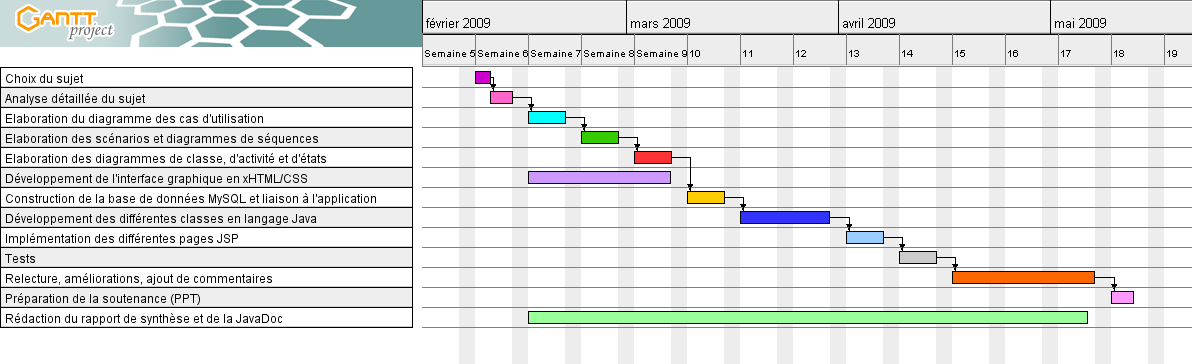
\includegraphics[scale=0.6]{./images/planning_projet_JAVA.png}
	\end{center}
	\begin{center}
	  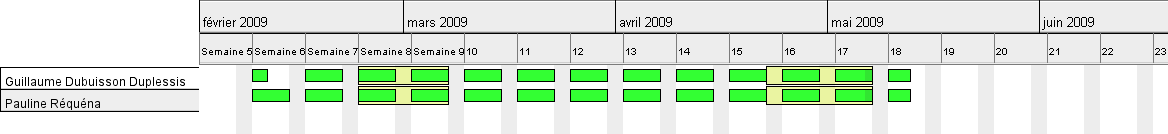
\includegraphics[scale=0.6]{./images/planning_projet_JAVA_res.png}
	\end{center}
\end{landscape}

\newpage
\section{Modélisation}
\subsection{Identification des acteurs}
Dans le cadre de  ce gestionnaire d'agendas, nous pouvons déterminer deux  principaux acteurs : l'utilisateur "lambda" qui gère  ses agendas et l'administrateur du site. Dans  un soucis de simplicité,
nous ne développerons pas l'administration du site. Nous ne considérerons donc pas l'administrateur.
\subsection{Diagramme de cas d'utilisation}
	\begin{center}
	  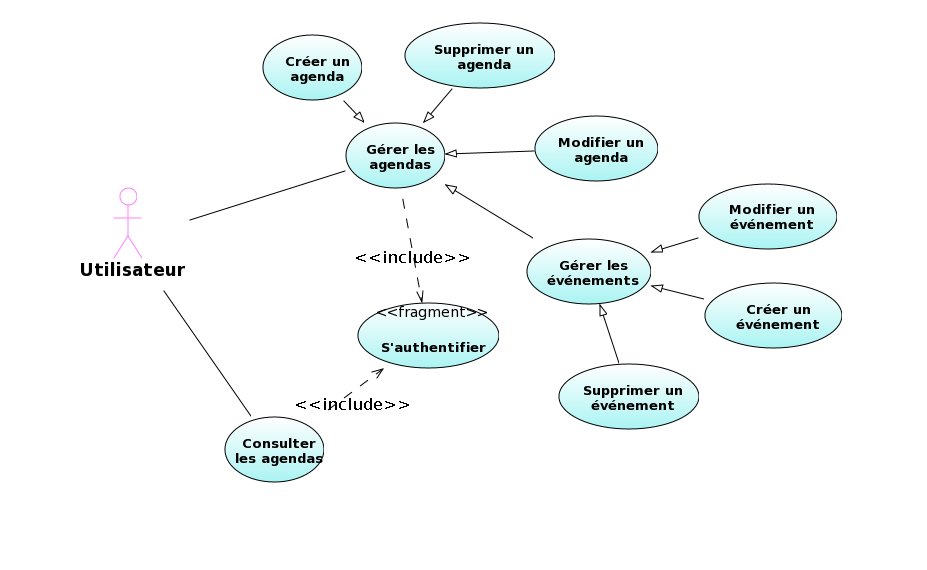
\includegraphics[scale=0.6]{./images/use_cases.png}
	\end{center}
\noindent Nous pouvons remarquer qu'il  n'apparaît pas de scénario d'inscription au site internet. En effet,  nous préférons nous concentrer sur la gestion des agendas  en elle-même que sur la gestion
des membres.

\newpage
\subsection{Les scénarios détaillés}
\subsubsection{Scénario "s'authentifier"}

\noindent\textbf{Titre : } s'authentifier\\
\textbf{Résumé : } ce cas d'utilisation permet à l'utilisateur de s'authentifier\\
\textbf{Acteur : }utilisateur\\

\noindent\textbf{Préconditions :}
\begin{itemize}
\item L'utilisateur n'est pas déjà authentifié
\item La base de données stockant la liste utilisateur/mot de passe est accessible \\
\end{itemize}


\noindent\textbf{Scénario nominal :}
\begin{enumerate}
\item Le système demande à l'utilisateur un nom d'utilisateur et un mot de passe
\item L'utilisateur indique son nom d'utilisateur et son mot de passe
\item Le système vérifie qu'un utilisateur correspond au nom d'utilisateur
\item Le système vérifie que le mot de passe indiqué correspond au mot de passe associé au nom de l'utilisateur
\item Le système crée une session pour l'utilisateur \\
\end{enumerate}


\noindent\textbf{Encha\^inements alternatifs :}\\
\noindent\textit{A1 : nom d'utilisateur provisoirement erroné}\\
L'encha\^inement A1 démarre au point 3 du scénario nominal.
\begin{enumerate}
\item[4.] Le système indique à l'utilisateur que le nom d'utilisateur est erroné pour la première ou la deuxième fois
\item[5.] Le système incrémente le compteur des tentatives d'authentification
\end{enumerate}
Le scénario nominal reprend au point 1.\\


\noindent\textit{A2 : mot de passe provisoirement erroné}\\
L'encha\^inement A2 démarre au point 4 du scénario nominal.
\begin{enumerate}
\item[5.] Le système indique à l'utilisateur que le mot de passe est erroné pour la première ou la deuxième fois
\item[6.] Le système incrémente le compteur des tentatives d'authentification
\end{enumerate}
Le scénario nominal reprend au point 1.\\


\noindent\textbf{Encha\^inements d'erreur :}\\
\noindent\textit{E1 : nom d'utilisateur définitivement erroné}\\
L'encha\^inement E1 démarre au point 3 du scénario nominal.
\begin{enumerate}
\item[4.] Le système indique à l'utilisateur que le nom d'utilisateur est erroné pour la 3ème fois
\item[5.] Le système indique que toute tentative d'authentification sera refusée
\item[6.] Le système enregistre la machine comme étant bannie pour une durée déterminée (par exemple 1h)
\end{enumerate}


\noindent\textit{E2 : mot de passe définitivement erroné}\\
L'encha\^inement E2 démarre au point 4 du scénario nominal.
\begin{enumerate}
\item[5.] Le système indique à l'utilisateur que le mot de passe est erroné pour la 3ème fois
\item[6.] Le système indique que toute tentative d'authentification sera refusée
\item[7.] Le système enregistre la machine comme étant bannie pour une durée déterminée (par exemple 1h)
\end{enumerate}

\newpage
\subsubsection{Scénario "Création d'un nouvel agenda"}

\noindent\textbf{Titre : } Création d’un nouvel agenda\\
\textbf{Résumé : } Ce scénario permet à l’utilisateur de créer un nouvel agenda dans son calendrier.\\
\textbf{Acteur : }utilisateur\\

\noindent\textbf{Préconditions :}
\begin{itemize}
\item L'utilisateur est authentifié
\item La base de données stockant la table des agendas est accessible\\
\end{itemize}


\noindent\textbf{Scénario nominal :}
\begin{enumerate}
\item L’utilisateur indique qu'il souhaite créer un nouvel agenda 
\item Le système affiche le formulaire de création d’agendas.
\item L'utilisateur renseigne le formulaire avec le nom de l'agenda, le lieu, une description, et une couleur représentative
\item Le système vérifie que le champ "Nom" est bien renseigné
\item Le système vérifie qu’aucun agenda du même nom n’existe déjà dans la base
\item Le système crée un nouvel agenda dans la base de données.\\
\end{enumerate}


\noindent\textbf{Encha\^inements alternatifs :}\\
\noindent\textit{A1 : le champ nom est vide}\\
L'encha\^inement A1 démarre au point 4 du scénario nominal.
\begin{enumerate}
\item[5.] Le système indique à l’utilisateur que le champ « Nom » n’est pas rempli et que la création est donc impossible.
\end{enumerate}
Le scénario nominal reprend au point 2.\\


\noindent\textit{A2 : il y a déjà un agenda du même nom dans la base}\\
L'encha\^inement A2 démarre au point 5 du scénario nominal.
\begin{enumerate}
\item[6.] Le système indique à l’utilisateur que ce nom est déjà utilisé et qu’il doit en choisir un nouveau.
\end{enumerate}
Le scénario nominal reprend au point 2.\\

\newpage
\subsubsection{Scénario "Modifier les paramètres d'un agenda"}
\noindent\textbf{Titre : } Modification d’un agenda\\
\textbf{Résumé : } Ce scénario permet à l’utilisateur de modifier les caractéristiques d’un agenda existant, s’il veut par exemple changer sa couleur ou son nom.\\
\textbf{Acteur : }utilisateur\\

\noindent\textbf{Préconditions :}
\begin{itemize}
\item L’utilisateur est authentifié
\item L'agenda doit exister
\item La base de données stockant la table des agendas est accessible\\
\end{itemize}


\noindent\textbf{Scénario nominal :}
\begin{enumerate}
\item L’utilisateur indique qu'il souhaite modifier un de ses agendas
\item Le système affiche le formulaire de modification d’agendas
\item L’utilisateur sélectionne un agenda à modifier
\item Le système vérifie que l’agenda existe dans la base de données
\item Le système vérifie que l’agenda appartient bien à l’utilisateur
\item Le système va chercher dans la base les caractéristiques de l’agenda et les affiche dans le formulaire.
\item L’utilisateur renseigne les différents champs, suivant les modifications qu’il désire effectuer et clique sur « Modifier ».
\item Le système vérifie que le champ « Nom » est bien renseigné.
\item Le système vérifie qu’aucun agenda du même nom n’existe pas déjà dans la base.
\item Le système modifie les informations de l’agenda dans la base de données\\
\end{enumerate}

\noindent\textbf{Encha\^inements alternatifs :}\\
\noindent\textit{A1 : l’agenda n’existe pas}\\
L'encha\^inement A1 démarre au point 4 du scénario nominal.
\begin{enumerate}
\item[5.] Le système indique à l’utilisateur que l’agenda n’existe pas donc il n’y a pas de modification possible
\end{enumerate}
Le scénario nominal reprend au point 2.\\


\noindent\textit{A2 : l’agenda n’appartient pas à l’utilisateur}\\
L'encha\^inement A2 démarre au point 5 du scénario nominal.
\begin{enumerate}
\item[6.] Le système indique à l’utilisateur qu’il n’a pas l’autorisation de modifier cet agenda
\end{enumerate}
Le scénario nominal reprend au point 2.\\


\noindent\textit{A3 : le champ nom est vide}\\
L'encha\^inement A3 démarre au point 8 du scénario nominal.
\begin{enumerate}
\item[9.] Le système indique à l’utilisateur que le champ « Nom » n’est pas rempli et que la modification est donc impossible
\end{enumerate}
Le scénario nominal reprend au point 6.\\


\noindent\textit{A4 : il y a déjà un agenda du même nom dans la base}\\
L'encha\^inement A4 démarre au point 9 du scénario nominal.
\begin{enumerate}
\item[10.] Le système indique à l’utilisateur que ce nom est déjà utilisé et qu’il doit en choisir un nouveau
\end{enumerate}
Le scénario nominal reprend au point 6.\\

\newpage
\subsubsection{Scénario "Supprimer un agenda"}
\noindent\textbf{Titre : } Suppression d’un agenda\\
\textbf{Résumé : } Ce scénario permet à l’utilisateur de supprimer un agenda existant, s’il n’en a plus l’utilité. Cette action a pour conséquence de supprimer tous les évènements relatifs à cet agenda.\\
\textbf{Acteur : }utilisateur\\

\noindent\textbf{Préconditions :}
\begin{itemize}
\item L’utilisateur est authentifié
\item L'agenda doit exister
\item La base de données stockant la table des agendas et des événements est accessible\\
\end{itemize}


\noindent\textbf{Scénario nominal :}
\begin{enumerate}
\item L’utilisateur indique qu'il souhaite supprimer un agenda
\item Le système affiche le formulaire de modification d’agendas
\item L’utilisateur sélectionne un agenda à supprimer
\item Le système vérifie que l’agenda existe dans la base de données.
\item Le système vérifie que l’agenda appartient bien à l’utilisateur
\item Le système va chercher dans la base les caractéristiques de l’agenda et les affiche dans le formulaire.
\item L’utilisateur confirme la suppression
\item Le système supprime l’agenda dans la base de données, ainsi que tous les évènements liés à cet agenda \\
\end{enumerate}

\noindent\textbf{Encha\^inements alternatifs :}\\
\noindent\textit{A1 : l’agenda n’existe pas}\\
L'encha\^inement A1 démarre au point 4 du scénario nominal.
\begin{enumerate}
\item[5.] Le système indique à l’utilisateur que l’agenda n’existe pas donc il n’y a pas de modification possible
\end{enumerate}
Le scénario nominal reprend au point 2.\\


\noindent\textit{A2 : l’agenda n’appartient pas à l’utilisateur}\\
L'encha\^inement A2 démarre au point 5 du scénario nominal.
\begin{enumerate}
\item[6.] Le système indique à l’utilisateur qu’il n’a pas l’autorisation de modifier cet agenda
\end{enumerate}
Le scénario nominal reprend au point 2.\\

\newpage
\subsubsection{Scénario "Création d’un nouvel évènement"}
\noindent\textbf{Titre : } Création d’un nouvel évènement\\
\textbf{Résumé : } Ce scénario permet à l’utilisateur de créer un nouvel évènement dans un agenda de son calendrier\\
\textbf{Acteur : }utilisateur\\

\noindent\textbf{Préconditions :}
\begin{itemize}
\item L’utilisateur est authentifié
\item L'agenda doit exister
\item La base de données stockant la table des agendas et des événements est accessible\\
\end{itemize}


\noindent\textbf{Scénario nominal :}
\begin{enumerate}
\item L’utilisateur indique qu'il souhaite créer un nouvel événement
\item Le système affiche le formulaire de création d’évènement.
\item L’utilisateur renseigne le formulaire avec l’objet de l’évènement, la date, le lieu, les heures de début et de fin, l’agenda auquel il appartient, et une description
\item Le système vérifie que l’agenda sélectionné existe bien dans la base.
\item Le système vérifie que l’agenda sélectionné appartient bien à l’utilisateur.
\item Le système vérifie que les champs « Objet », « Date », « Heure de début » et « Heure de fin » sont bien renseignés.
\item Le système vérifie qu’aucun évènement du même agenda n’existe déjà dans la base sur une plage horaire commune.
\item Le système crée un nouvel évènement  dans la base de données.\\
\end{enumerate}

\noindent\textbf{Encha\^inements alternatifs :}\\
\noindent\textit{A1 : l’agenda n’existe pas}\\
L'encha\^inement A1 démarre au point 4 du scénario nominal.
\begin{enumerate}
\item[5.] Le système indique à l’utilisateur que l’agenda n’existe pas donc il n’y a pas de modification possible
\end{enumerate}
Le scénario nominal reprend au point 2.\\


\noindent\textit{A2 : l’agenda n’appartient pas à l’utilisateur}\\
L'encha\^inement A2 démarre au point 5 du scénario nominal.
\begin{enumerate}
\item[6.] Le système indique à l’utilisateur qu’il n’a pas l’autorisation de modifier cet agenda
\end{enumerate}
Le scénario nominal reprend au point 2.\\


\noindent\textit{A3: un champ obligatoire n'est pas renseigné}\\
L'encha\^inement A3 démarre au point 6 du scénario nominal.
\begin{enumerate}
\item[7.] Le système indique à l’utilisateur que certains des champs « Objet », « Date », « Heure de début » ou « Heure de fin » ne sont pas renseignés.
\end{enumerate}
Le scénario nominal reprend au point 2.\\


\noindent\textit{A4: un évènement simultané existe déjà}\\
L'encha\^inement A3 démarre au point 7 du scénario nominal.
\begin{enumerate}
\item[8.] Le système indique à l’utilisateur qu’il doit changer les horaires de son évènement car cette plage horaire est déjà occupée.
\end{enumerate}
Le scénario nominal reprend au point 2.\\


\newpage
\subsubsection{Scénario "Modifier les détails d'un évènement"}
\noindent\textbf{Titre : } Modification d’un évènement\\
\textbf{Résumé : } Ce scénario permet à l’utilisateur de modifier les détails d’un évènement existant dans un agenda de son calendrier. Il peut par exemple vouloir changer la plage horaire d’un rendez-vous, ou le lieu d’une soirée etc.\\
\textbf{Acteur : }utilisateur\\

\noindent\textbf{Préconditions :}
\begin{itemize}
\item L’utilisateur est authentifié
\item L'agenda doit exister
\item La base de données stockant la table des agendas et des événements est accessible\\
\end{itemize}


\noindent\textbf{Scénario nominal :}
\begin{enumerate}
\item L’utilisateur sélectionne l’évènement qu’il veut modifier.
\item Le système vérifie que l’évènement sélectionné existe bien dans la base.
\item Le système vérifie que l’évènement sélectionné appartient bien à l’utilisateur.
\item Le système va chercher dans la base les caractéristiques de l’évènement et affiche le formulaire de modification d’évènement.
\item L’utilisateur renseigne le formulaire en modifiant les champs voulus et clique sur le bouton « Modifier ».
\item Le système vérifie que les champs « Objet », « Date », « Heure de début » et « Heure de fin » sont bien renseignés.
\item Le système vérifie qu’aucun évènement du même agenda n’existe déjà dans la base sur une plage horaire commune.
\item Le système modifie les caractéristiques de l’évènement dans la base de données.\\
\end{enumerate}

\noindent\textbf{Encha\^inements alternatifs :}\\
\noindent\textit{A1 : l’événement n’existe pas}\\
L'encha\^inement A1 démarre au point 4 du scénario nominal.
\begin{enumerate}
\item[5.] Le système indique à l’utilisateur que l’événement n’existe pas donc il n’y a pas de modification possible
\end{enumerate}
Le scénario nominal reprend au point 1.\\


\noindent\textit{A2 : l’événement n’appartient pas à l’utilisateur}\\
L'encha\^inement A2 démarre au point 3 du scénario nominal.
\begin{enumerate}
\item[6.] Le système indique à l’utilisateur qu’il n’a pas l’autorisation de modifier cet événement
\end{enumerate}
Le scénario nominal reprend au point 1.\\


\noindent\textit{A3: un champ obligatoire n'est pas renseigné}\\
L'encha\^inement A3 démarre au point 6 du scénario nominal.
\begin{enumerate}
\item[7.] Le système indique à l’utilisateur que certains des champs « Objet », « Date », « Heure de début » ou « Heure de fin » ne sont pas renseignés.
\end{enumerate}
Le scénario nominal reprend au point 5.\\

\noindent\textit{A4 : un évènement simultané existe déjà}\\
L’enchaînement A4 démarre au point 7 du scénario nominal.
\begin{enumerate}
\item[8.] Le système indique à l’utilisateur qu’il doit changer les horaires de son évènement car cette plage horaire est déjà occupée.
\end{enumerate}
Le scénario nominal revient au point 5.\\




\newpage
\subsubsection{Scénario "Supprimer un évènement"}
\noindent\textbf{Titre : } Suppression d’un évènement\\
\textbf{Résumé : } Ce scénario permet à l’utilisateur de supprimer un évènement existant\\
\textbf{Acteur : }utilisateur\\

\noindent\textbf{Préconditions :}
\begin{itemize}
\item L’utilisateur est authentifié
\item L'agenda doit exister
\item La base de données stockant la table des agendas et des événements est accessible\\
\end{itemize}


\noindent\textbf{Scénario nominal :}
\begin{enumerate}
\item L’utilisateur sélectionne l’évènement qu’il veut modifier
\item Le système vérifie que l’évènement existe dans la base de données
\item Le système vérifie que l’évènement appartient bien à l’utilisateur
\item Le système va chercher dans la base les caractéristiques de l’évènement sélectionné et les affiche dans le formulaire
\item L’utilisateur clique sur « Supprimer »
\item Le système supprime l’évènement  de la base de données\\
\end{enumerate}

\noindent\textbf{Encha\^inements alternatifs :}\\
\noindent\textit{A1 : l’événement n’existe pas}\\
L'encha\^inement A1 démarre au point 2 du scénario nominal.
\begin{enumerate}
\item[5.] Le système indique à l’utilisateur que l’événement n’existe pas donc il n’y a pas de modification possible
\end{enumerate}
Le scénario nominal reprend au point 1.\\


\noindent\textit{A2 : l’événement n’appartient pas à l’utilisateur}\\
L'encha\^inement A2 démarre au point 3 du scénario nominal.
\begin{enumerate}
\item[6.] Le système indique à l’utilisateur qu’il n’a pas l’autorisation de modifier cet événement
\end{enumerate}
Le scénario nominal reprend au point 1.\\

\subsection{Diagramme d'activité}
\noindent Nous avons vu les différents scénarios du projet, nous allons maintenant voir les différents diagrammes d'activité correspondant.

\subsubsection{Authentification}
\begin{center}
  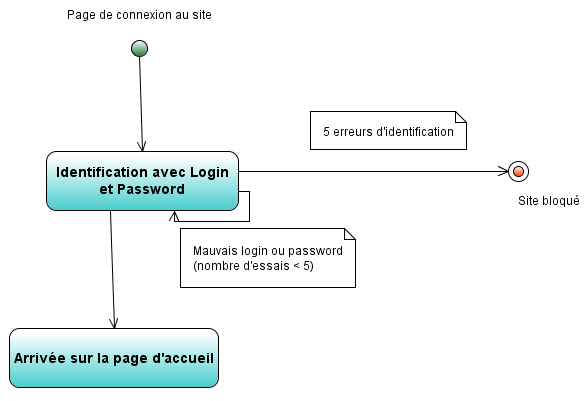
\includegraphics[scale=0.6]{./images/diag_act_authentification.png}
\end{center}
\noindent Comme nous pouvons le voir sur ce diagramme, l'utilisateur indique son login et son mot de passe. Il a 5 tentatives pour arriver à se connecter, après quoi il n'aura plus accès à la connexion.

\subsubsection{Création d'agenda}
\begin{center}
  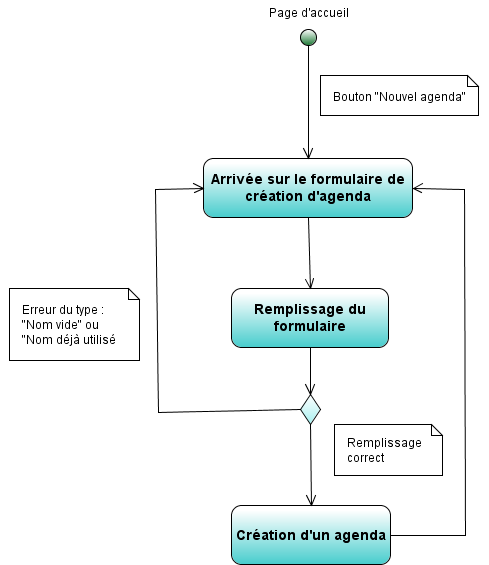
\includegraphics[scale=0.6]{./images/diag_act_creation_agenda.png}
\end{center}
\noindent Comme nous pouvons le voir sur ce diagramme, la création d'un agenda consiste en  le remplissage d'un formulaire. Les données communiquées par le formulaire sont vérifiés. Dans le cas où ces
données seraient erronées (nom vide ou déjà utilisé), l'utilisateur est invité à remplir de nouveau le formulaire.
Enfin si le formulaire est correctement rempli, l'agenda est créé.

\subsubsection{Création d'événement}
\begin{center}
  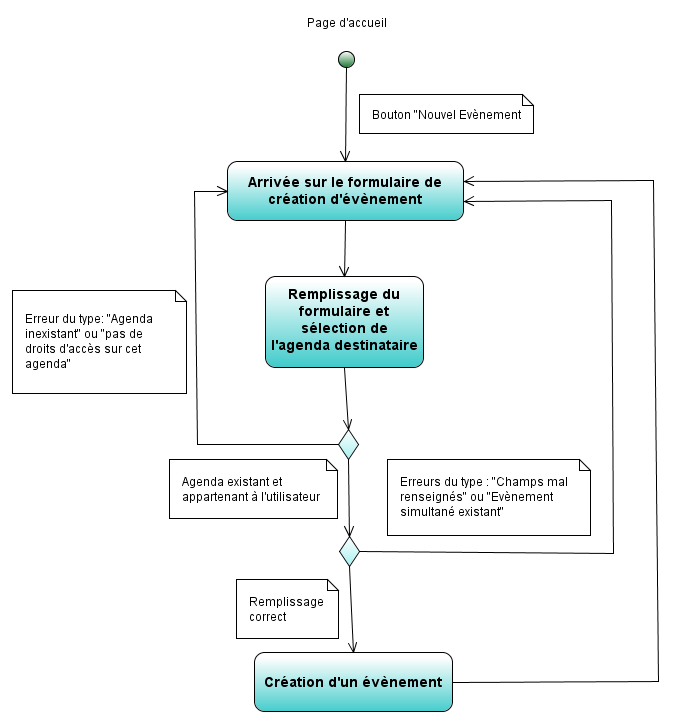
\includegraphics[scale=0.6]{./images/diag_act_creation_evenement.png}
\end{center}
\noindent De la m\^eme manière que la création d'agenda, l'utilisateur est invité à remplir un formulaire pour créer des événements. L'événement est créé quand toutes les conditions sont remplies :
champs bien renseignés, aucun événement simultané n'existe, l'agenda dans lequel l'utilisateur souhaite ajouter un événement lui appartient.

\subsubsection{Modification d'agenda}
\begin{center}
  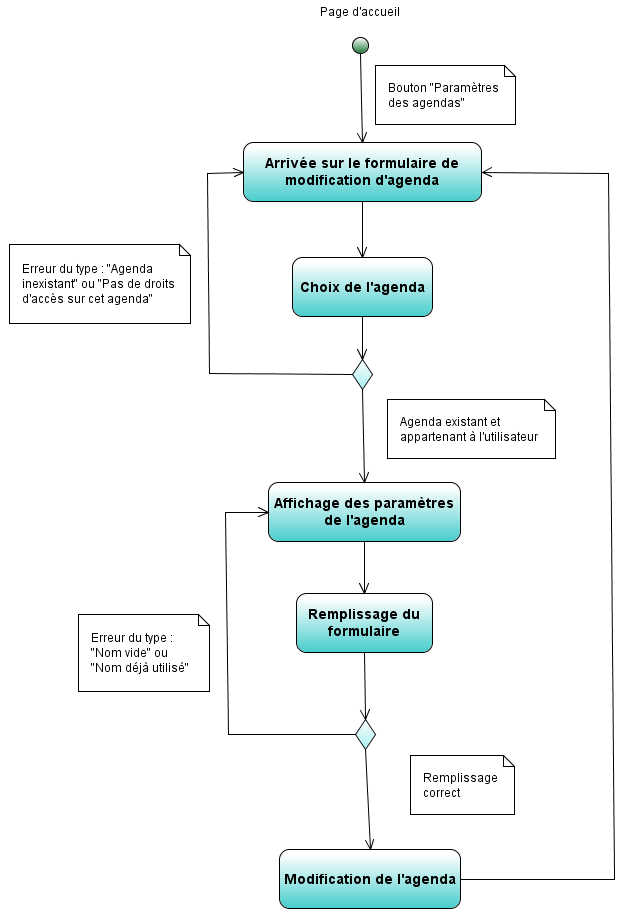
\includegraphics[scale=0.6]{./images/diag_act_modification_agenda.png}
\end{center}

\subsubsection{Modification d'événement}
\begin{center}
  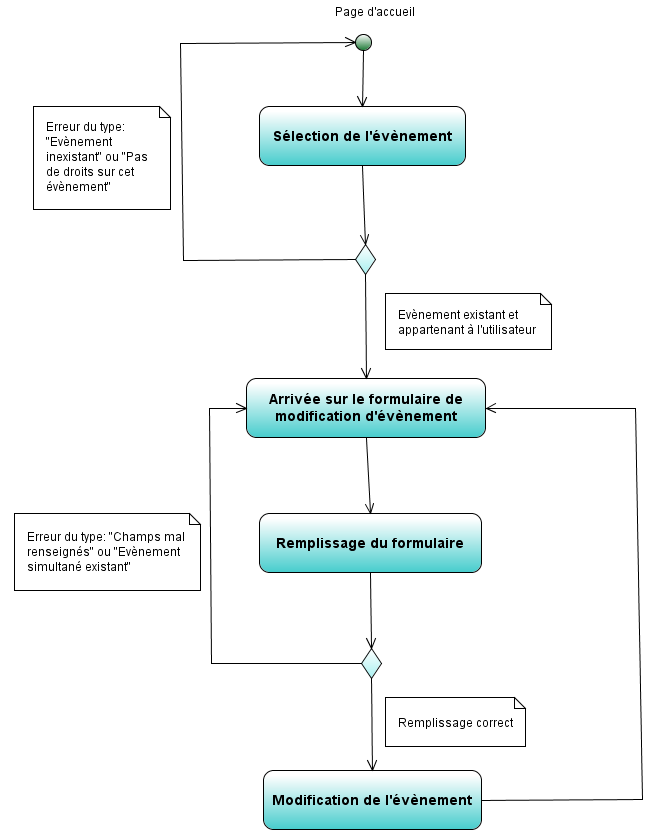
\includegraphics[scale=0.6]{./images/diag_act_modification_evenement.png}
\end{center}
\newpage

\subsubsection{Suppression d'agenda}
\noindent La suppression d'un agenda s'effectue de la façon suivante :
\begin{center}
  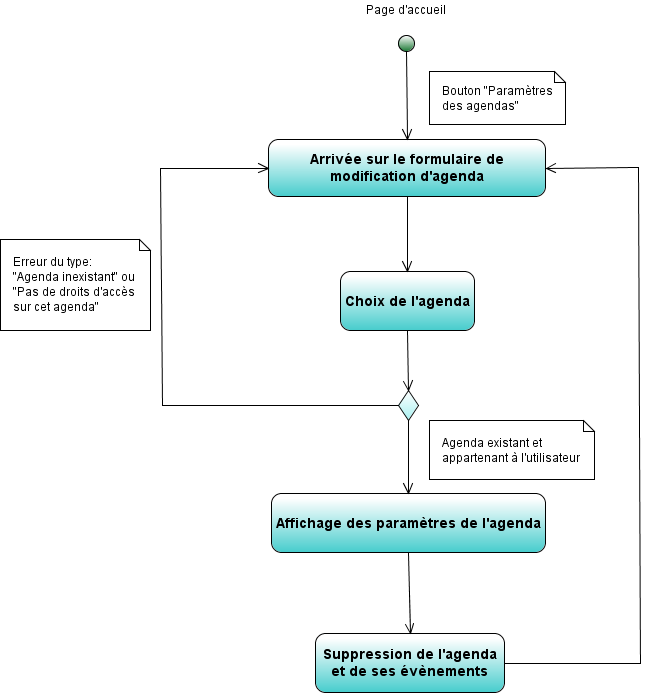
\includegraphics[scale=0.6]{./images/diag_act_suppression_agenda.png}
\end{center}
\noindent 
\newpage

\subsubsection{Suppression d'événement}
\noindent Lorsqu'un utilisateur souhaite supprimer un événement, cela se passe de la manière suivante :
\begin{center}
  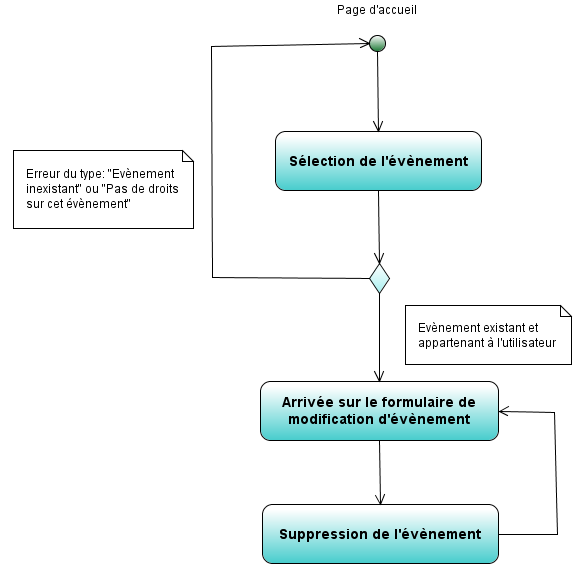
\includegraphics[scale=0.6]{./images/diag_act_suppression_evenement.png}
\end{center}

\begin{landscape}
\subsubsection{Diagramme d'activité global}
\begin{center}
  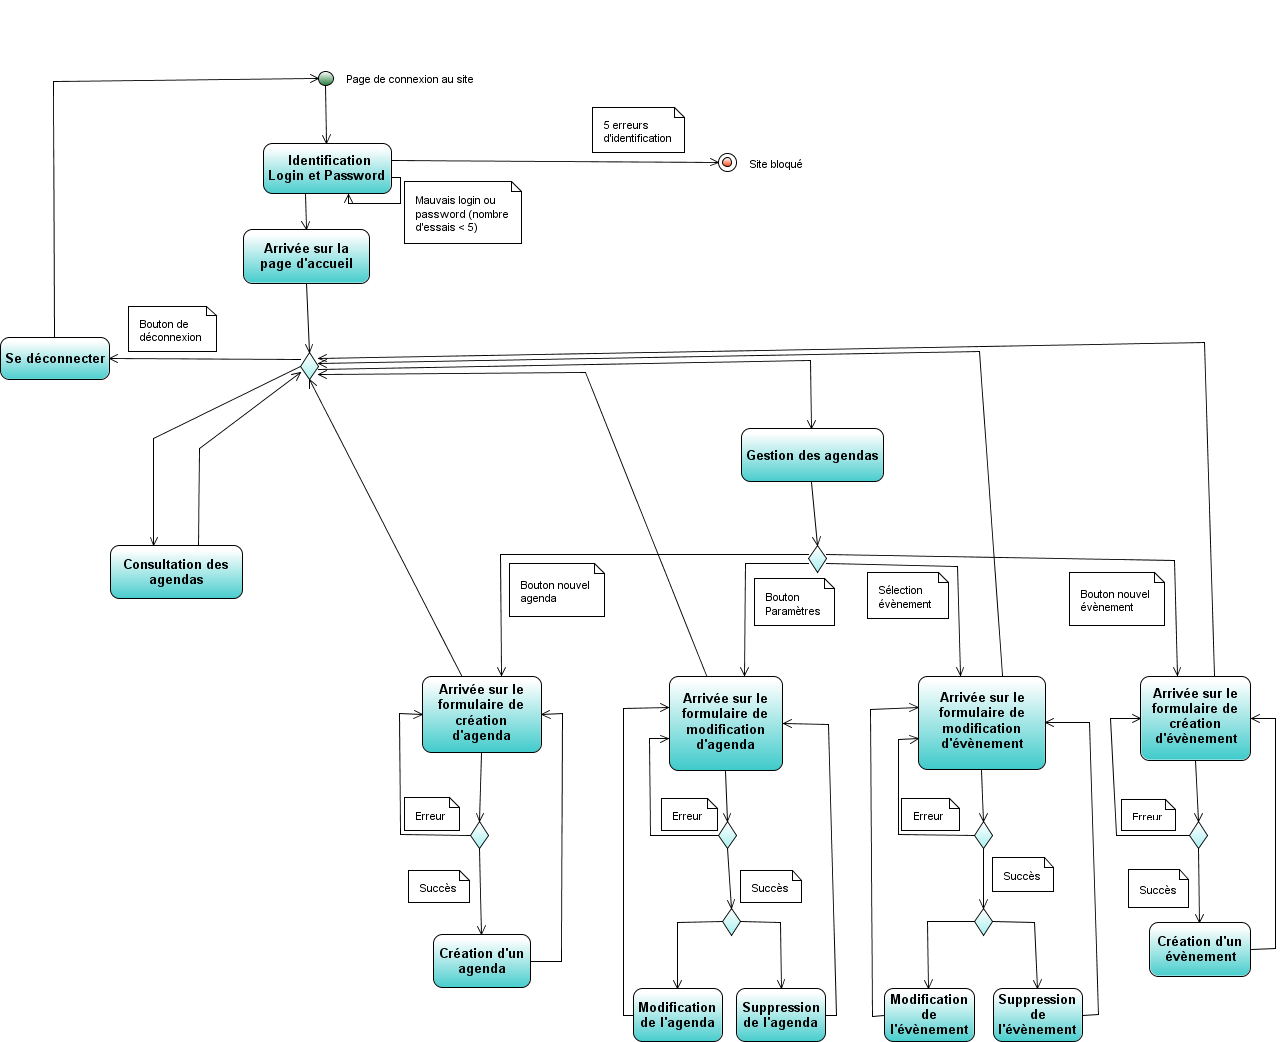
\includegraphics[scale=0.45]{./images/diag_activite.png}
\end{center}
\end{landscape}

\subsection{Diagramme de séquences}
\noindent Nous allons maintenant voir les différents diagrammes de séquences qui permettent de décrire les interactions entre les objets de notre projet.
\subsubsection{Authentification}
\noindent Ce premier diagramme définit l'authentification. Celle-ci est finalement très simple puisque qu'il s'agit d'une interrogation d'un objet UtilisateurDAO (DAO pour Data Access Object) qui
permet de s'abstraire de la façon dont sont stockées les données référençant l'utilisateur.\\
Dans le cas où l'utilisateur n'existe pas ou que le mot de passe ne correspond pas, un signal est envoyé par UtilisateurDAO.
\begin{center}
  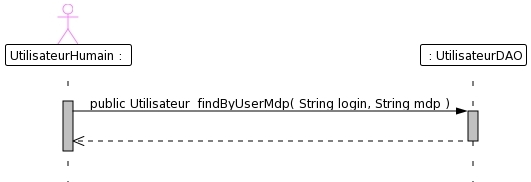
\includegraphics[scale=0.55]{./images/diag_seq_authentification.jpg}
\end{center}


\begin{landscape}
\subsubsection{Creer un agenda}
\noindent Un  des points clé de  notre projet est la  création d'agenda. Ce diagramme  de séquence explique  le déroulement de cette  opération. Comme nous pouvons  le voir ci-dessous, la  création de
l'agenda commence par  l'ajout dans le portefeuille d'agendas  de l'utilisateur qui vérifiera que  le nom de l'agenda est  valide et qu'il n'est pas  déjà attribué. Si toutes les  conditions sont bien
remplies, l'agenda est alors ajouté au portefeuille.\\
Bien entendu la persistance de cette modification sera assurée par un objet PortefeuilleAgendaDAO qui appelera également des objets AgendaDAO et EvenementDAO.
\begin{center}
  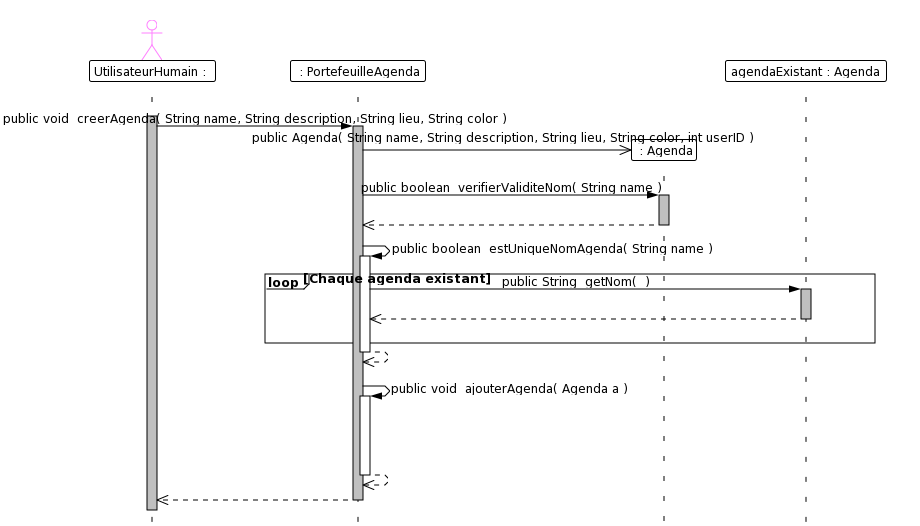
\includegraphics[scale=0.55]{./images/diag_seq_creer_agenda.png}
\end{center}
\end{landscape}

\begin{landscape}
\subsubsection{Modifier un agenda}
\noindent Après avoir  ajouté un agenda, l'utilisateur  doit toujours \^etre capable de  le modifier. Ce diagramme  explique le déroulemet de cette  opération. On constatera qu'il  s'agit de récupérer
l'agenda correspondant dans le portefeuille d'agenda puis de le modifier en vérifiant bien sur que les nouvelles données correspondent aux conditions décrites dans les scénarios.
\begin{center}
  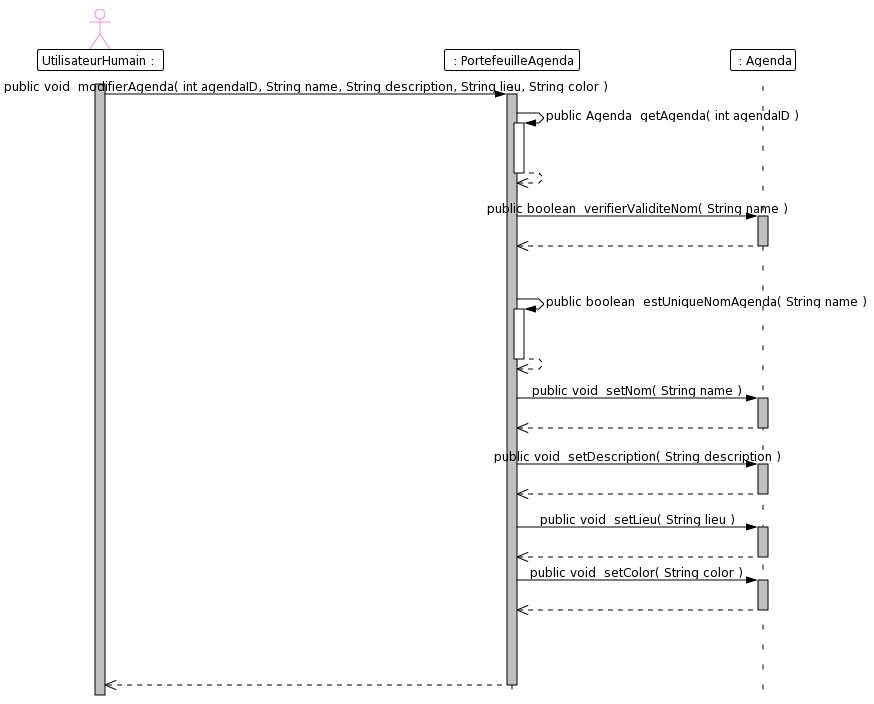
\includegraphics[scale=0.55]{./images/diag_seq_modifier_agenda.jpg}
\end{center}
\end{landscape}

\begin{landscape}
\subsubsection{Supprimer un agenda}
\noindent Un utilisateur peut également supprimer un agenda. Ce diagramme de séquence décrit le déroulement de cette opération.
\begin{center}
  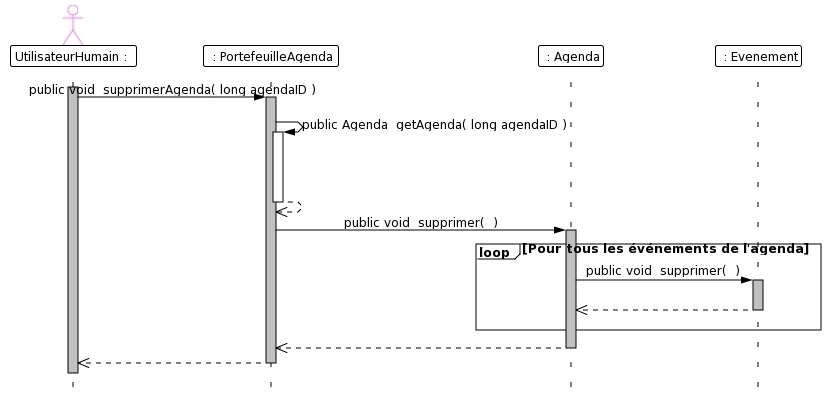
\includegraphics[scale=0.55]{./images/diag_seq_supprimer_agenda.jpg}
\end{center}
\end{landscape}

\begin{landscape}
\subsubsection{Création d'un événement}
\noindent Une fois que l'utilisateur possède un ou plusieurs agendas, il peut ajouter des événements. L'ajout d'événement est décrit par le diagramme de séquence suivant :
\begin{center}
  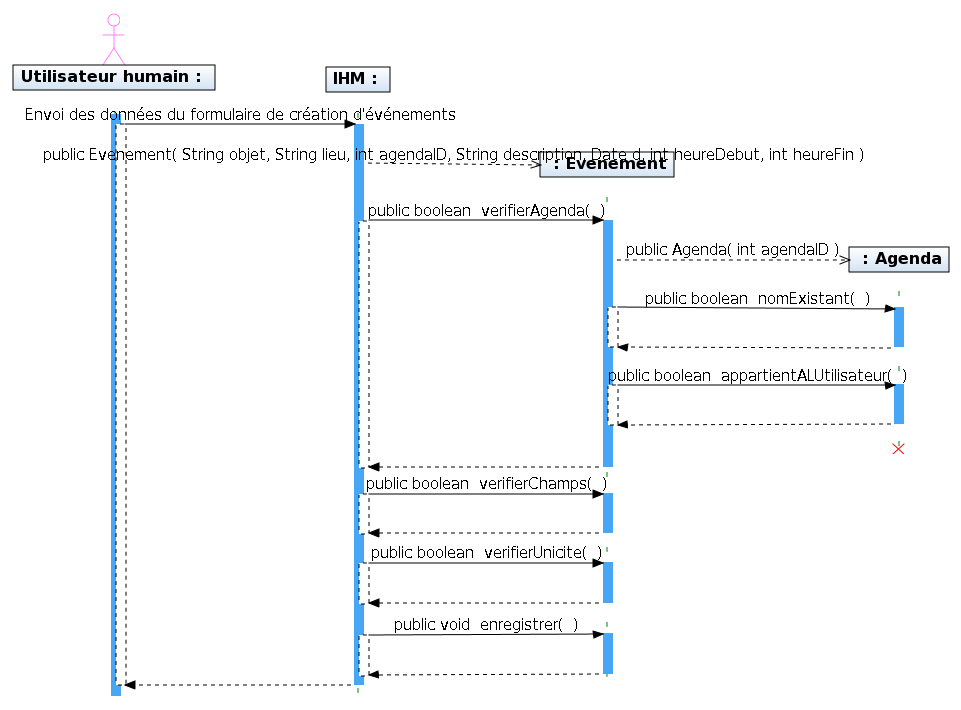
\includegraphics[scale=0.55]{./images/diag_seq_creation_evenement.png}
\end{center}
\noindent Il faut souligner que dans  un m\^eme agenda, il ne peut pas y avoir plusieurs  événements sur un m\^eme créneau horaire. Nous avons choisi cette option  pour des raisons de simplicité d'une
part et parce que l'utilisateur peut très bien créer un autre événement simultané dans un autre agenda.
\end{landscape}

\begin{landscape}
\subsubsection{Modifier un événement}
\noindent L'utilisateur peut bien évidemment modifier un événement qu'il a créé. Cette opération s'effectue selon le diagramme de séquence suivant :
\begin{center}
  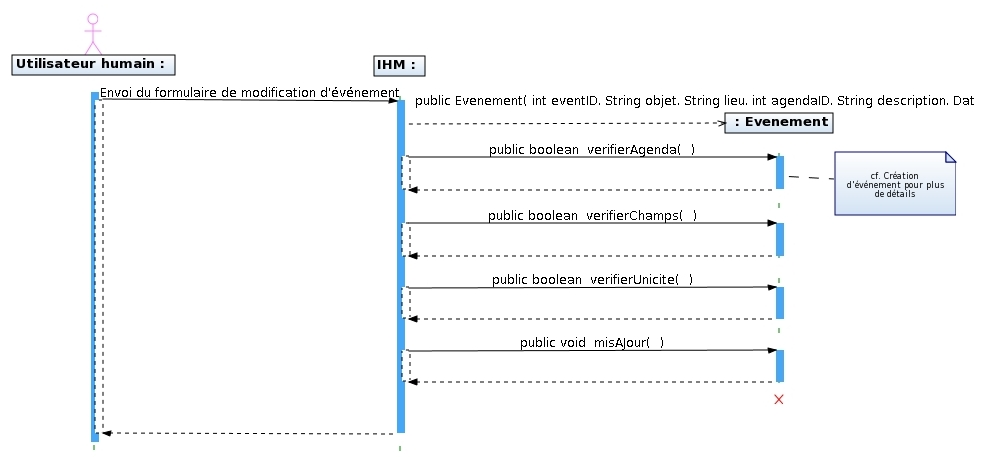
\includegraphics[scale=0.55]{./images/diag_seq_modifier_evt.jpg}
\end{center}
\end{landscape}

\begin{landscape}
\subsubsection{Supprimer un événement}
\noindent Finalement, un utilisateur peut supprimer un événement. Cette opération s'effecture selon le diagramme de séquence suivant :
\begin{center}
  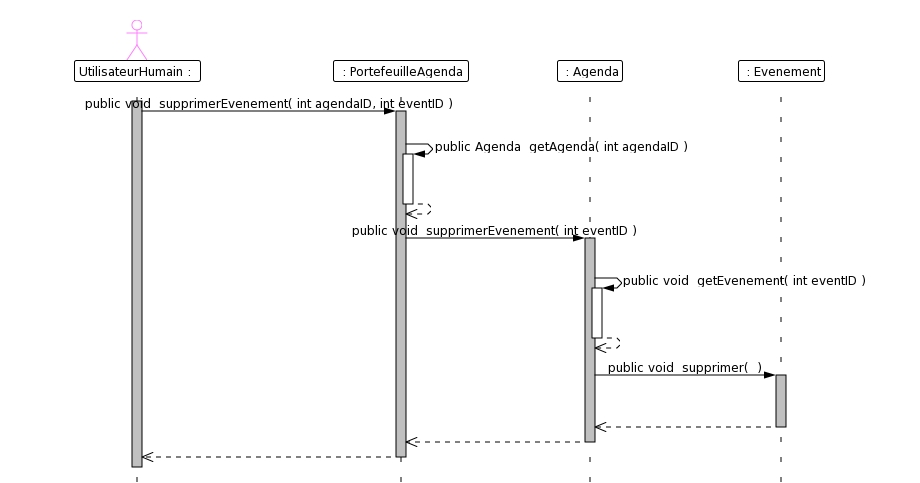
\includegraphics[scale=0.55]{./images/diag_seq_supprimer_evt.jpg}
\end{center}
\end{landscape}

\subsection{Diagramme de classes}
\noindent Nous allons maintenant voir la décomposition en différentes classes que nous avons choisie.

\subsubsection{Gestionnaire d'agendas}
\noindent Les premières classes sont directement en rapport avec le gestionnaire d'agenda. Il s'agit de nos classes métiers.
\begin{itemize}
\item PortefeuilleAgenda : associé à un utilisateur, il regroupe les agendas et permet des opérations telles que l'ajout, la modification et la suppression d'agendas et d'événements
\item Agenda : associé  à un utilisateur, il regroupe les différents  événements ajoutés. Il permet l'ajout, la modification  et la suppression d'événements. Un agenda est caractérisé  par un nom, une
  description, une couleur et un lieu.
\item Evenement : caractérisé par un objet, un lieu, une description et une date de début et de fin
\end{itemize}
\noindent Toutes ces classes sont regroupées dans le paquetage "Gestion agenda".
\begin{center}
  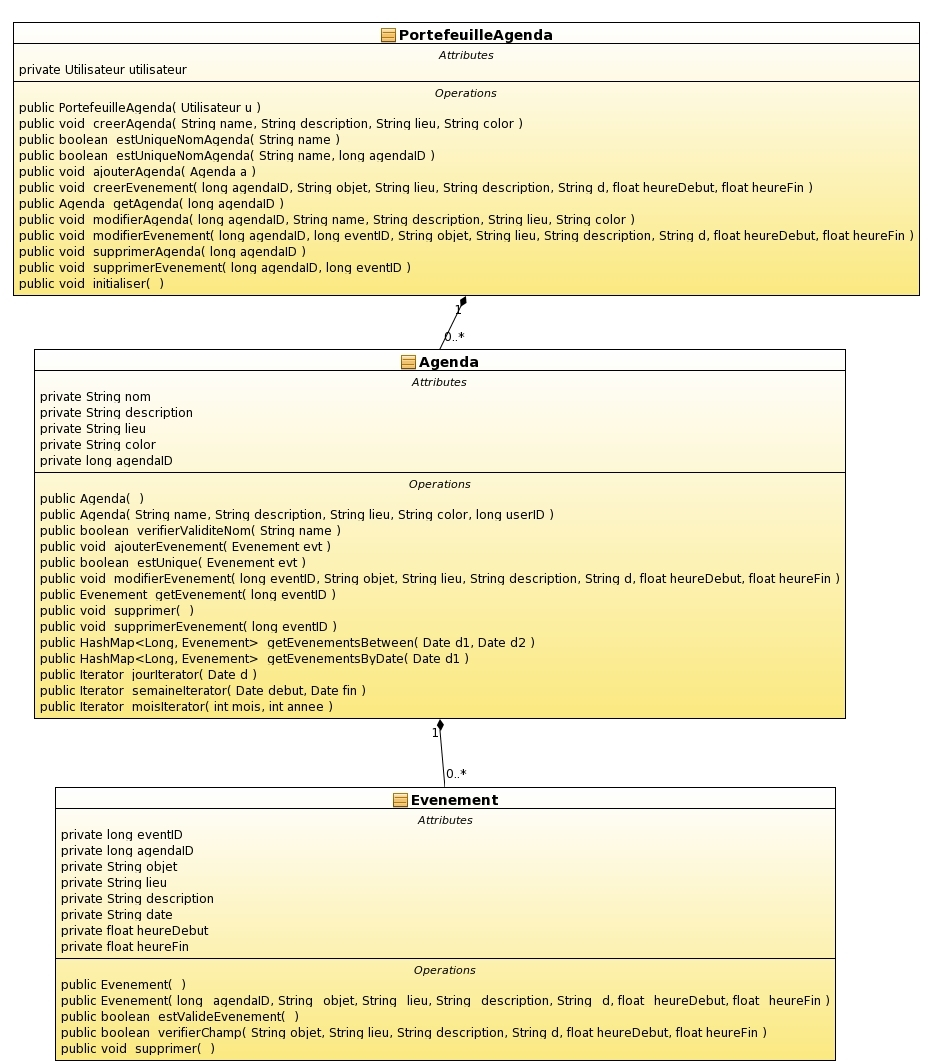
\includegraphics[scale=0.45]{./images/class_diagram_gestionagenda.jpg}
\end{center}


\subsubsection{Authentification}
\noindent Pour accéder à ses agendas, l'utilisateur  doit s'authentifier à l'aide d'un couple pseudonyme (ou login) / mot de passe. Cette authentification  est rendue persistante grace à un système de
Session qui intègre des options de sécurité (une session ne peut exister plus d'un certain temps, une session inactive trop longtemps n'est plus valide).
D'où les deux classes :
\begin{itemize}
\item Utilisateur : caractérisé par un login, mot de passe et un identifiant unique
\item Session : caractérisé par un identifiant unique, une date de début, une date de dernière activité, une adresse IP et bien évidemment un utilisateur
\end{itemize}
\noindent Ces classes sont regroupées dans le paquetage "Authentification" et sont réutilisables pour n'importe quel autre projet.

\begin{center}
  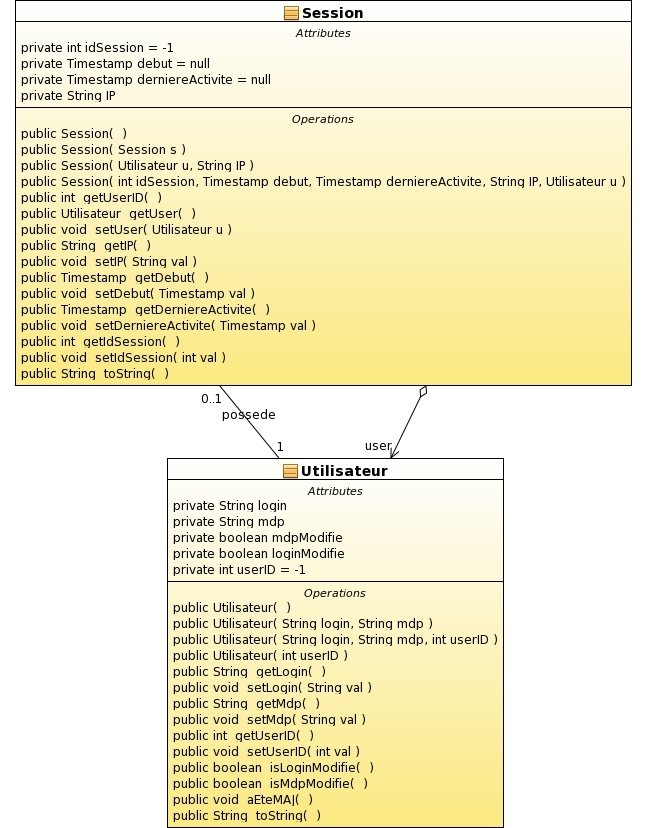
\includegraphics[scale=0.5]{./images/class_diagram_authentification.jpg}
\end{center}

\newpage
\subsubsection{Service DAO}
\noindent Enfin, pour assurer la persistance des objets  nous avons créé des interfaces DAO qui permettent le mapping entre les objets manipulés par  le programme et un système de stockage (comme une
base de données, des fichiers XML). Il y a une classe DAO pour chaque classe que nous avons vu précédemment.\\
Ces interfaces sont regroupées dans le paquetage "Service".\\
Dans le cadre de notre projet, nous avons implémenté ces différentes interfaces pour réaliser un mapping objet/mySQL.
\begin{center}
  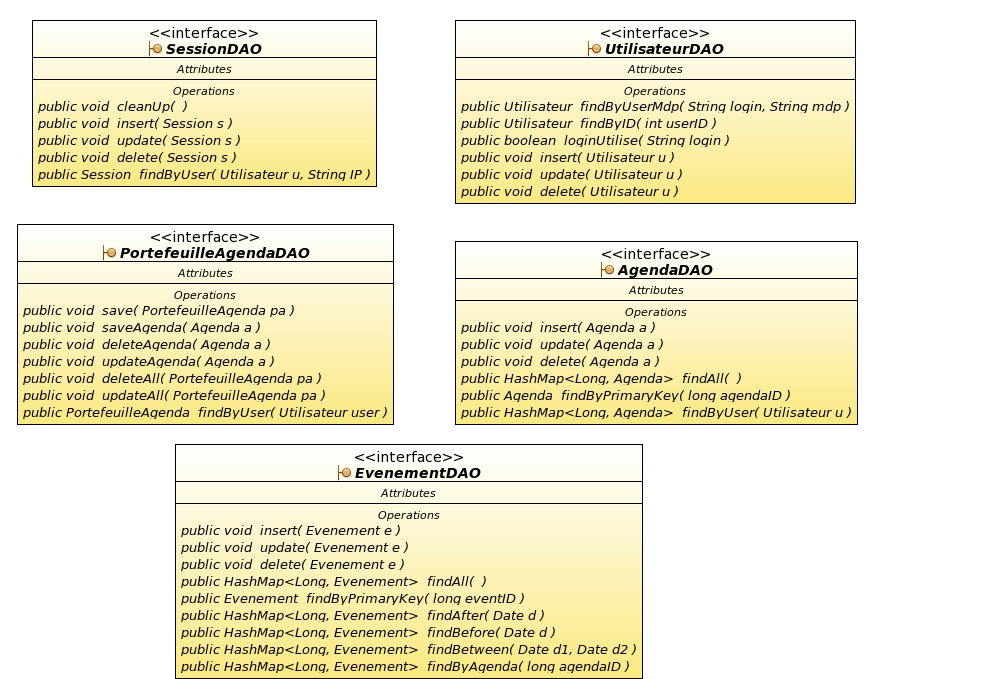
\includegraphics[scale=0.5]{./images/class_diagram_DAO.jpg}
\end{center}

\newpage
\subsubsection{Les différents paquetages}
\noindent Voici les différents paquetages utilisés lors de notre projet. Le contenu des  paquetages GestionAgenda, Authentification, et service a été décrit précédemment. Le paquetage sql contenu dans
le paquetage service est l'implémentation des interfaces DAO pour le mapping objet/mySQL.
\begin{center}
  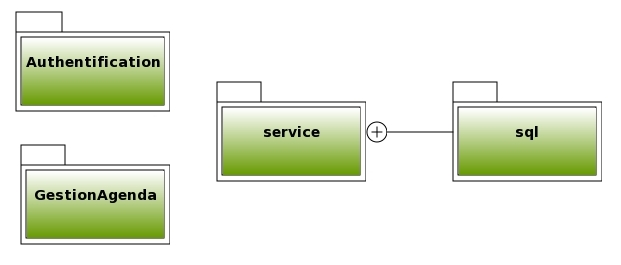
\includegraphics[scale=0.5]{./images/paquetages.jpg}
\end{center}

\newpage
\subsection{Modèle E/A et relationnel de la base de données}

\subsubsection{Modèle entité/association}
\noindent Pour modéliser notre base de données, nous nous sommes appuyés sur le modèle entité/association suivant :
\begin{center}
  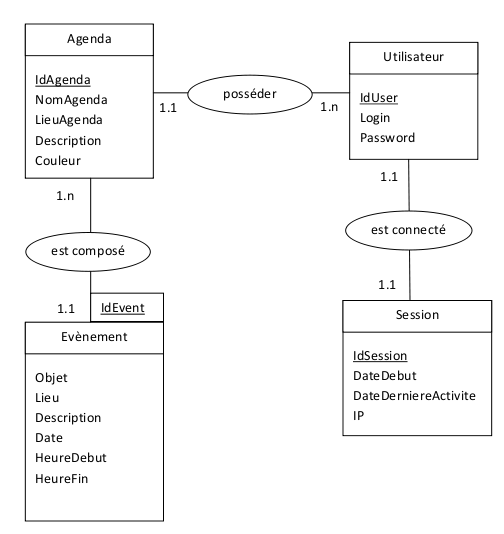
\includegraphics[scale=0.8]{./images/EA.png}
\end{center}

\noindent Comme  nous pouvons le voir,  un utilisateur est connecté  à une Session. En  fait, cette session se  comporte comme une persistance  de l'authentification. Un  utilisateur possède plusieurs
agendas qui contiennent eux-m\^emes des événements.\\
Nous allons maintenant passer à la transformation vers le modèle relationnel.

\subsubsection{Modèle relationnel}
\paragraph{Pour chaque entité, on crée une relation \\}
\noindent Agenda(\textbf{IdAgenda},NomAgenda,LieuAgenda,Description,Couleur)\\
Utilisateur(\textbf{IdUser},Login,Password) \\
Session(\textbf{IdSession},DateDebut,DateDerniereActivite,IP)

\paragraph{Entité faible\\}
\noindent Evènement est une entité faible d'Agenda. On crée donc un mécanisme de clé étrangère pour
référencer l'entité forte dans l'entité faible.\\
Evènement(\textbf{IdAgenda},\textbf{IdEvent},Objet,Lieu,Description,Date,HeureDebut,HeureFin)

\paragraph{Autres associations binaires\\}
\noindent L'identifiant de l'utilisateur devient un attribut de la table Agenda.\\
L'identifiant de l'utilisateur devient un attribut de la table Session.\\ \\

\noindent On obtient ainsi le modèle relationnel suivant :\\
Agenda(\textbf{IdAgenda},NomAgenda,LieuAgenda,Description,Couleur,IdUser)\\
Utilisateur(\textbf{IdUser},Login,Password)\\
Session(\textbf{IdSession},DateDebut,DateDerniereActivite,IP,IdUser)\\
Evènement(\textbf{IdAgenda},\textbf{IdEvent},Objet,Lieu,Description,Date,HeureDebut,HeureFin)\\
\begin{center}
  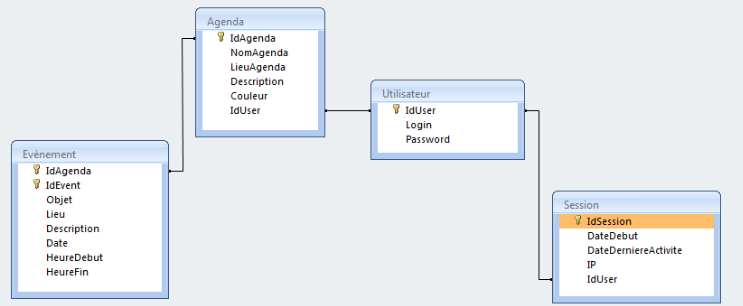
\includegraphics[scale=0.6]{./images/relationnel.png}
\end{center}


\newpage
\section{Exemple de fonctionnement}
\subsection{Identification}
\noindent Lorsque l’utilisateur veut se connecter à l’application, il est dirigé vers la page d’identification
du gestionnaire d’agendas.\\
L’identification se fait grâce à un nom d’utilisateur et un mot de passe stockés dans la base de
données de l’application. L’utilisateur doit donc remplir les champs « Nom d’utilisateur » et
« Mot de passe » avec ses identifiants et cliquer ensuite sur le bouton « Se connecter ».

\begin{center}
  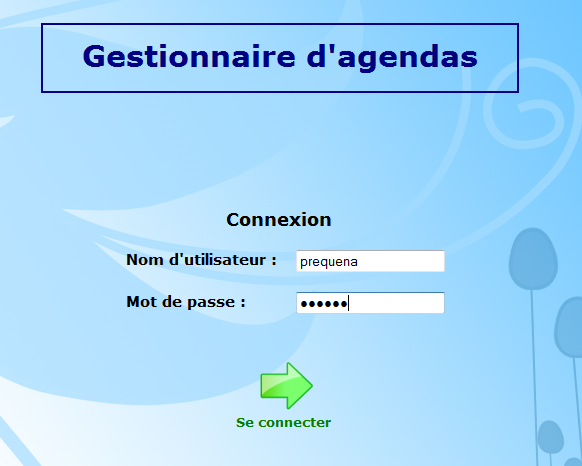
\includegraphics[scale=0.6]{./images/authentification2.png}
\end{center}

\subsubsection{Authentification réussie}
\noindent Si un utilisateur correspondant à ce couple login/mot de passe est enregistré dans la base et si
aucune session n’est déjà ouverte pour cet utilisateur, l’authentification est réussie et
l’utilisateur arrive sur la page de bienvenue :

\begin{center}
  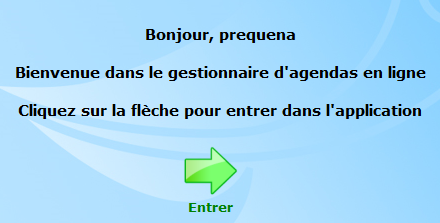
\includegraphics[scale=0.6]{./images/authentification4.png}
\end{center}

\noindent Il doit ensuite cliquer sur le bouton « Entrer » pour finalement entrer dans le gestionnaire
d’agendas.

\subsubsection{Erreurs d'authentification}
\noindent Il existe plusieurs types d’erreurs d’authentification :
\begin{itemize}
\item Couple login/mot de passe inexistant
\item 5 échecs de connexion
\item Session déjà ouverte pour cet utilisateur
\end{itemize}

\paragraph{Couple login/mot de passe inexistant\\}
 Si aucun utilisateur de la base ne correspond au nom d’utilisateur et au mot de passe, entrés
dans les champs d’identification, un message d’erreur est affiché et l’utilisateur est redirigé vers
la page d’authentification.

\begin{center}
  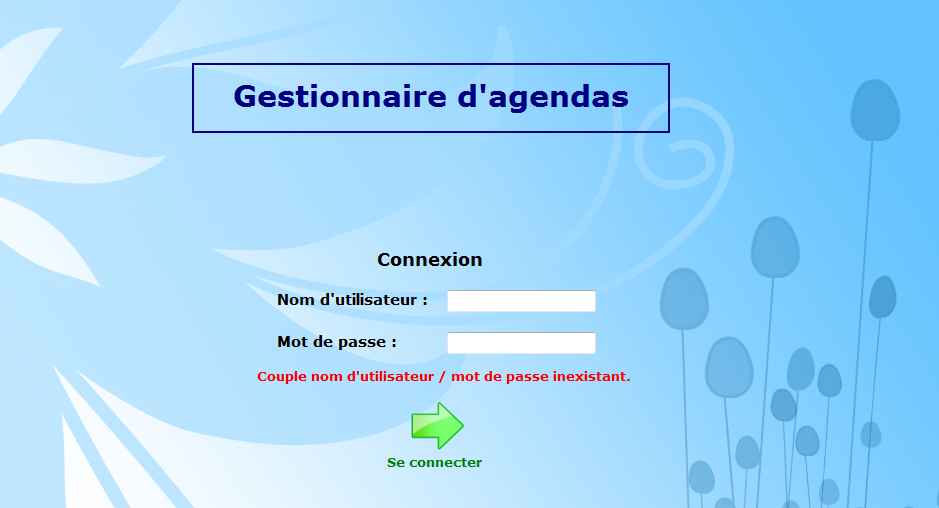
\includegraphics[scale=0.6]{./images/authentification3.png}
\end{center}


\paragraph{5 échecs de connexion\\}
Au bout de 5 tentatives de connexion infructueuses, l’accès à l’application est bloqué.
L’utilisateur ne peut plus accéder à la page de connexion pour des raisons de sécurité. Cette
mesure évite que certaines personnes puissent tomber par hasard sur un couple login/mot de
passe valide, en essayant de multiples valeurs et ainsi pirater le compte d’un autre utilisateur.

\begin{center}
  
\includegraphics[scale=0.6]{./images/authentification5.png}
\end{center}

\newpage
\subsection{Page d'accueil : structure et fonctionnement}
\noindent Une fois l’authentification réussie, l’utilisateur arrive sur la page d’accueil de l’application.

\begin{center}
  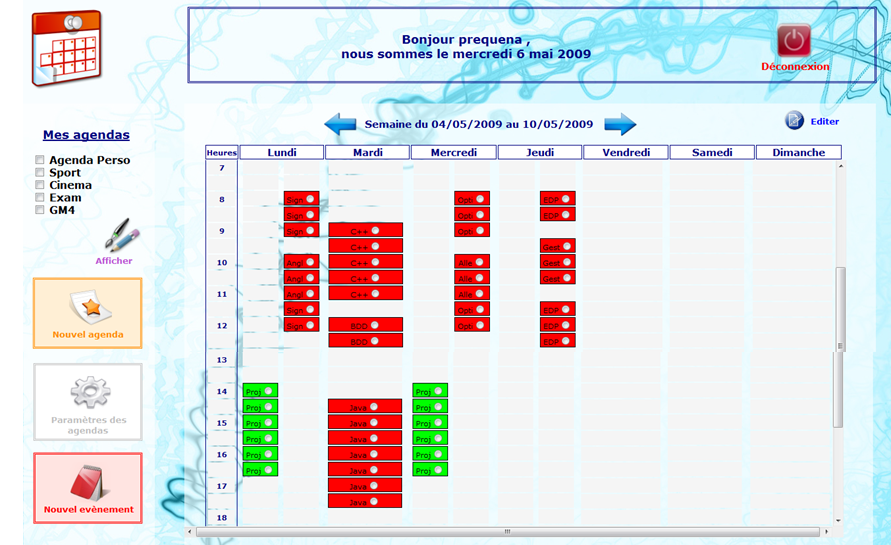
\includegraphics[scale=0.6]{./images/accueil3.png}
\end{center}


\noindent Cette page est composée de 3 parties :
\subsubsection{Le menu horizontal }
\noindent Ce menu est constitué du logo de l’application, et d’un cadre possédant :
\begin{itemize}
\item un message d’accueil pour l’utilisateur connecté
\item une indication de la date du jour
\item  un bouton permettant de se déconnecter de l’application
\end{itemize}

\begin{center}
  
\includegraphics[scale=0.4]{./images/accueil4.png}
\end{center}



\subsubsection{Le menu vertical de gauche}
\noindent Ce menu est composé de 2 parties :
\begin{itemize}
\item   Une liste des agendas de l’utilisateur
\end{itemize}

\begin{center}
  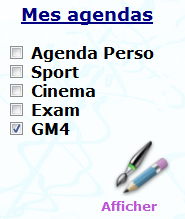
\includegraphics[scale=0.6]{./images/calendrier_agenda3.png}
\end{center}

\noindent Ce dernier peut choisir ceux qu’il souhaite voir apparaître dans
son calendrier en les sélectionnant et en cliquant sur le bouton
« Afficher ».

\newpage

\begin{itemize}
\item Des boutons d’accès aux différentes pages de gestion des agendas et des évènements
\end{itemize}

\begin{center}
  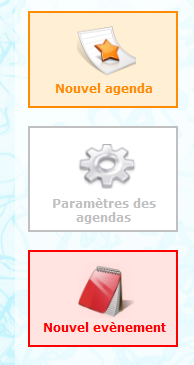
\includegraphics[scale=0.6]{./images/accueil5.png}
\end{center}       

\noindent Le bouton « Nouvel agenda » permet d’accéder au
formulaire de création d’un agenda.\\
\noindent Le bouton « Paramètres des agendas » permet d’accéder au
formulaire de modification ou de suppression d’un agenda.\\
\noindent Le bouton « Nouvel évènement » permet d’accéder au
formulaire de création d’un évènement.\\





\subsubsection{Le calendrier d'affichage des agendas}
\noindent Ce calendrier permet à l’utilisateur connecté de consulter ces agendas par semaine.\\ \\
Lorsque l’utilisateur se connecte à l’application, la semaine par défaut est la semaine
correspondant à la date du jour. Mais il lui est ensuite possible de changer en utilisant les
flèches bleues situées de part et d’autre de la semaine courante, qui permettent de passer à la
semaine précédente ou à la semaine suivante. \\ \\
Dans le calendrier, les agendas sont affichés sont ceux sélectionnés dans la liste « Mes agendas »
du menu vertical de gauche (cf. paragraphe précédant). Pour plus de visibilité, chaque agenda
a une couleur caractéristique. Par exemple, dans le screenshot ci-dessous, l’agenda « Cinéma »
est caractérisé par la couleur bleu clair, et l’agenda « GM4 » est caractérisé par la couleur
rouge.

\begin{center}
  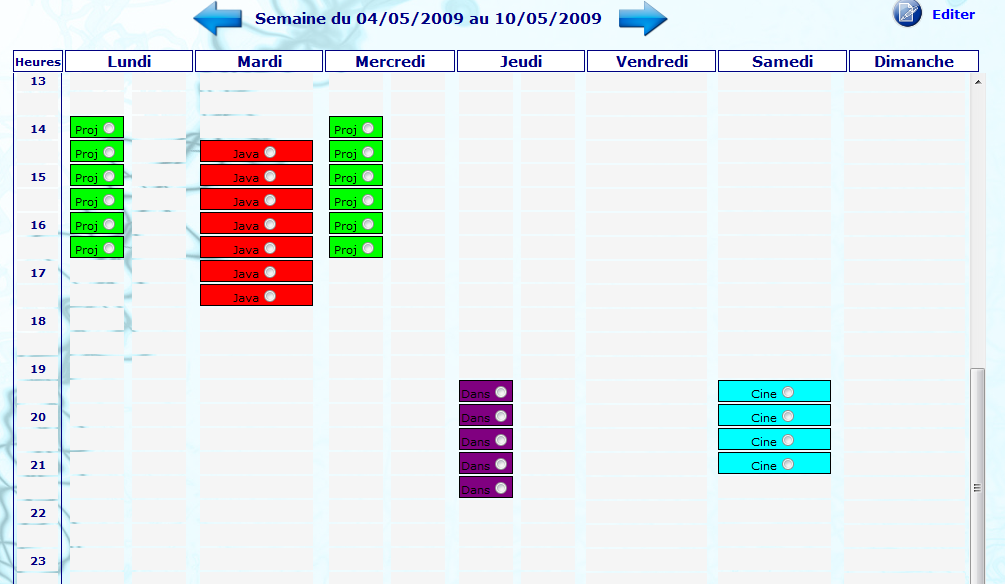
\includegraphics[scale=0.6]{./images/calendrier_agenda.png}
\end{center}


\noindent Si l’utilisateur choisit de ne sélectionner que l’agenda « GM4 »,
\begin{center}
  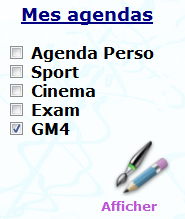
\includegraphics[scale=0.6]{./images/calendrier_agenda3.png}
\end{center}
\noindent son calendrier aura donc l’allure suivante :
\begin{center}
  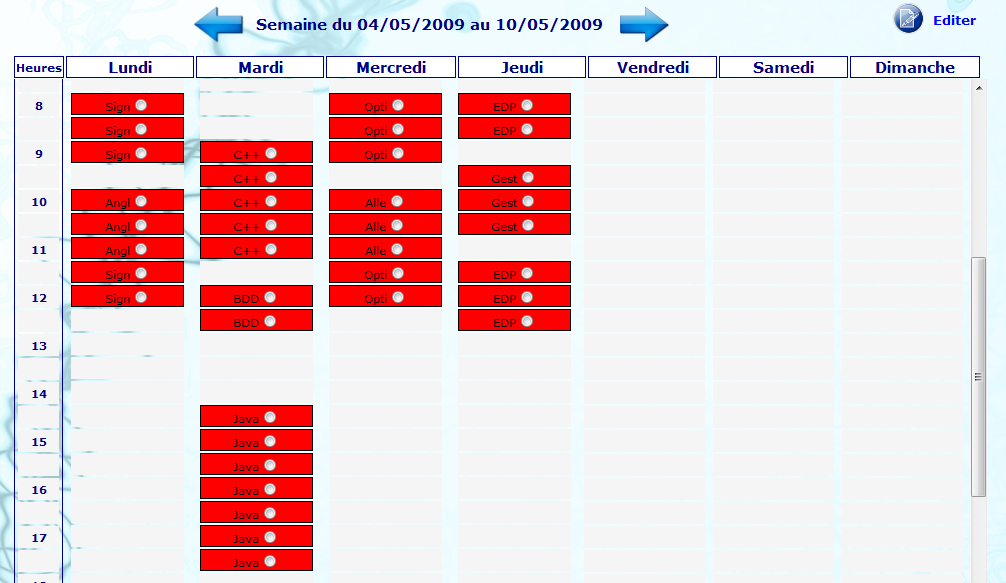
\includegraphics[scale=0.6]{./images/calendrier_agenda2.png}
\end{center}



\noindent Pour modifier un évènement, l’utilisateur doit le sélectionner en cochant le bouton radio
correspondant et ensuite cliquer sur le bouton « Editer », situé en haut à droite du calendrier.












\subsection{Créer un agenda}
\noindent Pour créer un agenda, l’utilisateur doit cliquer sur le bouton « Nouvel Agenda » du menu
vertical de gauche. Il est ensuite dirigé sur le formulaire suivant :
\begin{center}
  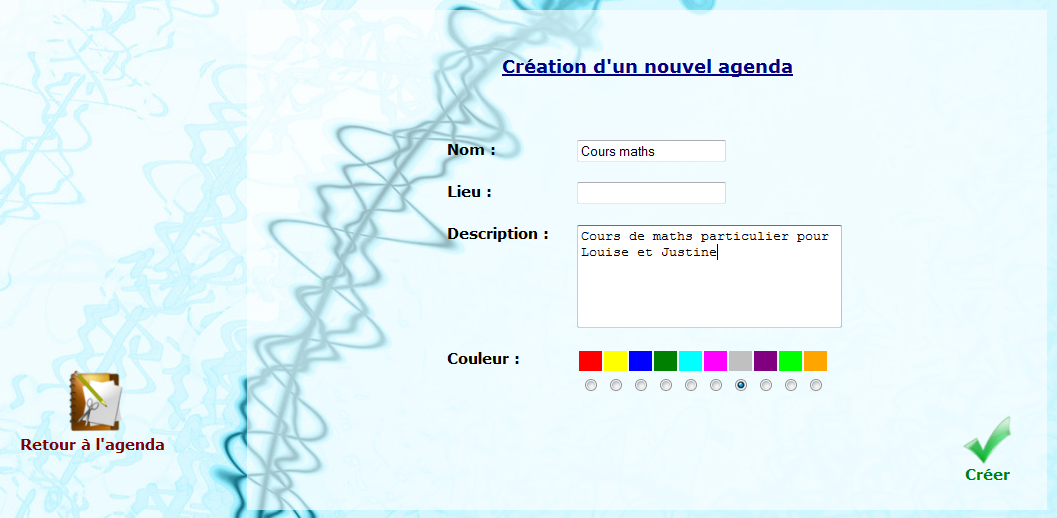
\includegraphics[scale=0.6]{./images/creation_agenda1.png}
\end{center}





\noindent Un agenda est caractérisé par les 4 informations suivantes :
\begin{itemize}
\item un nom
\item un lieu d'application
\item une description
\item une couleur d'affichage
\end{itemize}
L’utilisateur doit donc renseigner ce formulaire de création et ensuite cliquer sur le bouton
« Créer » pour le valider.


\subsubsection{Création réussie}
\noindent Si l’utilisateur a rempli correctement le formulaire, i.e. s’il a au moins rempli le champ « Nom »
avec une valeur valide, la création est effectuée et un message d’information est affiché.
\begin{center}
  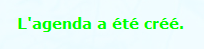
\includegraphics[scale=0.8]{./images/creation_agenda2.png}
\end{center}


\subsubsection{Erreurs de création}
\noindent Si l’utilisateur n’a pas rempli le champ « Nom » du formulaire, la création est invalidée et un
message d’erreur est affiché.
\begin{center}
  
\includegraphics[scale=0.8]{./images/creation_agenda3.png}
\end{center}


\noindent Si l’utilisateur possède un autre agenda portant le même nom que celui inscrit dans le champ
« Nom » du formulaire, la création est invalidée et un message d’erreur est affiché.
\begin{center}
  
\includegraphics[scale=0.8]{./images/creation_agenda4.png}
\end{center}




\noindent L’utilisateur peut à tout moment retourner sur la page d’accueil en cliquant sur le bouton
« Retour à l’agenda ».





\subsection{Modifier les paramètres d'un agenda}
\noindent Pour modifier les paramètres d’un agenda, l’utilisateur doit cliquer sur le bouton « Paramètres
des agendas » du menu vertical de gauche. Il est ensuite dirigé sur le formulaire suivant :
\begin{center}
  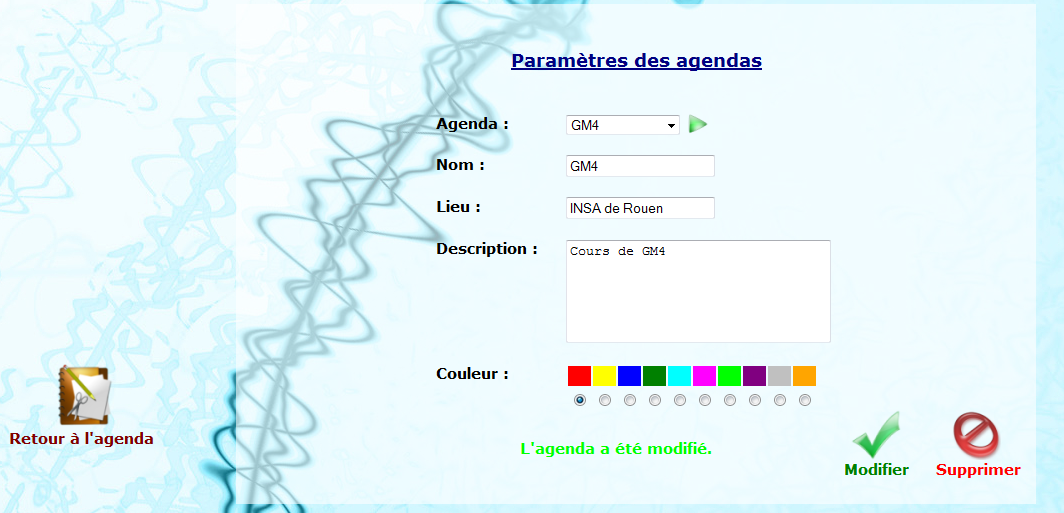
\includegraphics[scale=0.6]{./images/param_agenda3.png}
\end{center}

\noindent Il doit tout d’abord sélectionner l’agenda qu’il désire modifier en le sélectionnant dans la liste
déroulante « Agenda » et en cliquant ensuite sur la flèche verte. Les caractéristiques de l’agenda
sélectionné sont ainsi affichées dans les différents champs du formulaire.

\subsubsection{Suppression de l'agenda}
\noindent Pour supprimer l’agenda sélectionné, l’utilisateur doit cliquer sur le bouton « Supprimer » situé
en bas à droite du formulaire. Cette action a pour conséquence de supprimer l’agenda de la
base de données, ainsi que tous les évènements relatifs à cet agenda.
\begin{center}
  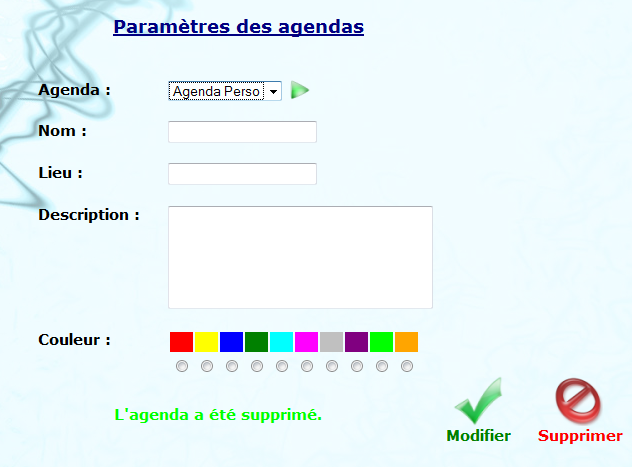
\includegraphics[scale=0.6]{./images/param_agenda1.png}
\end{center}

\subsubsection{Modification des caractéristiques de l'agenda}
\noindent Pour modifier les caractéristiques de l’agenda sélectionné l’utilisateur doit renseigner les
champs du formulaire avec les informations voulues et cliquer ensuite sur le bouton
« Modifier ». Si le formulaire a été correctement rempli, la modification est validée et un
message d’information est affiché.

\begin{center}
  
\includegraphics[scale=0.6]{./images/modif_agenda.png}
\end{center}



\noindent \textbf{NB :} La modification est invalidée dans le cas d’erreurs de même type que lors de la création
d’un agenda, à savoir le champ « Nom » non rempli, ou un agenda portant déjà le nom inscrit
dans le champ « Nom ».



\subsection{Créer un événement}
\noindent Pour créer un nouvel évènement, l’utilisateur doit cliquer sur le bouton «Nouvel Evènement »
du menu vertical de gauche. Il est ensuite dirigé sur le formulaire suivant :
\begin{center}
  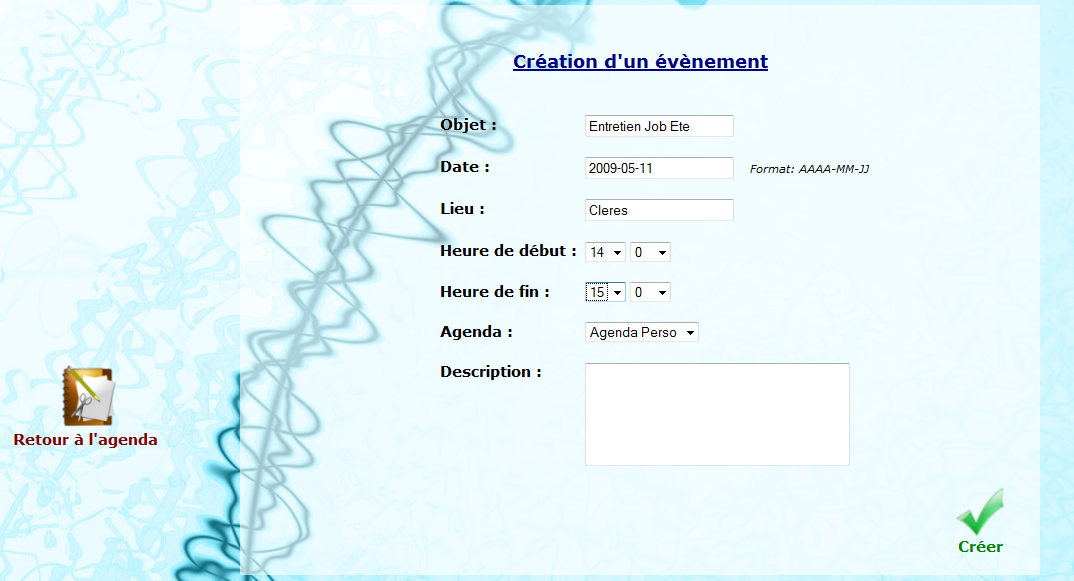
\includegraphics[scale=0.4]{./images/creation_event1.png}
\end{center}




Un évènement est caractérisé par les 7 informations suivantes :
\begin{itemize}
\item L’agenda auquel il appartient
\item Un objet
\item Une date d’application
\item Un lieu d’application
\item Une heure de début
\item Une heure de fin
\item Une description
\end{itemize}
         

\noindent L’utilisateur doit donc renseigner ce formulaire de création et ensuite cliquer sur le bouton
« Créer » pour le valider.






\subsubsection{Création réussie}
\noindent Si l’utilisateur a rempli correctement le formulaire, i.e. s’il a au moins rempli les champs
« Agenda », « Objet », « Date », « Heure de début » et « Heure de fin » avec des valeurs valides,
la création est effectuée et un message d’information est affiché.
\begin{center}
  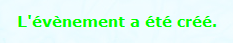
\includegraphics[scale=0.6]{./images/creation_event2.png}
\end{center}



\subsubsection{Erreurs de création}
\noindent Le premier type d’erreur de création correspond à un mauvais remplissage des champs par
l’utilisateur, à savoir :

\begin{itemize}
\item   Champ « Objet » non rempli
\item Date invalide
\item Heures de début de fin invalides : heure de début supérieure à l'heure de fin
\end{itemize}

\noindent Dans l’un de ces 3 cas, la création est invalidée et un message d’erreur est affiché.

\begin{center}
  
\includegraphics[scale=0.6]{./images/creation_event3.png}
\end{center}



\noindent Le second type d’erreur de création correspond à l’existence dans l’agenda sélectionné, d’un
évènement simultané, i.e. possédant une date et des heures de début et de fin identiques. Dans
ce cas, la création est invalidée et un message d’erreur est affiché.

\begin{center}
  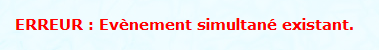
\includegraphics[scale=0.6]{./images/creation_event4.png}
\end{center}


\subsection{Modifier les paramètres d'un événement}
\noindent Pour modifier les paramètres d’un évènement, l’utilisateur doit le sélectionner dans le
calendrier de la page d’accueil et cliquer sur le bouton « Editer ». Il est ensuite dirigé sur le
formulaire suivant :
\begin{center}
  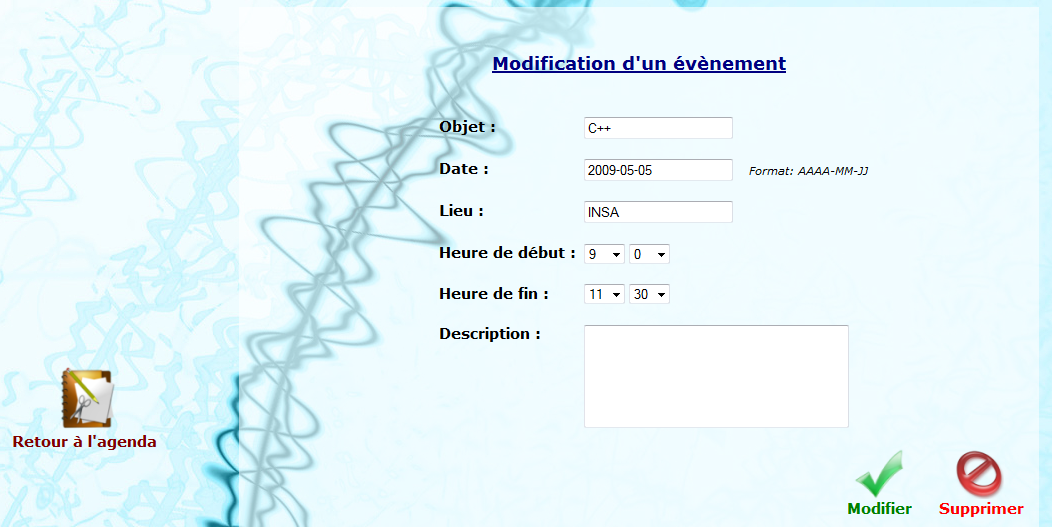
\includegraphics[scale=0.6]{./images/modif_event.png}
\end{center}




\noindent Les caractéristiques de l’évènement sélectionné sont affichées dans les différents champs du
formulaire.\\ \\
\textbf{NB} : L’utilisateur ne peut pas déplacer son évènement d’un agenda à l’autre. C’est pour cette
raison que le champ « Agenda » n’apparaît pas dans ce formulaire. Pour déplacer un
évènement vers un autre agenda, l’utilisateur doit le supprimer du premier agenda, et ensuite
le recréer dans un autre agenda.

\subsubsection{Suppresion de l'événement}
\noindent Pour supprimer l’évènement sélectionné, l’utilisateur doit cliquer sur le bouton « Supprimer »
situé en bas à droite du formulaire. Cette action a pour conséquence de supprimer
l’évènement de la base de données.
\begin{center}
  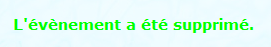
\includegraphics[scale=0.6]{./images/modif_event3.png}
\end{center}



\subsubsection{Modification des caractéristiques de l'événement}
\noindent Pour modifier les caractéristiques de l’évènement sélectionné, l’utilisateur doit renseigner les
champs du formulaire avec les informations voulues et cliquer ensuite sur le bouton
« Modifier ». Si le formulaire a été correctement rempli, la modification est validée et un
message d’information est affiché.
\begin{center}
  
\includegraphics[scale=0.6]{./images/modif_event2.png}
\end{center}


\noindent \textbf{NB} : La modification est invalidée dans le cas d’erreurs de même type que lors de la création
d’un évènement, à savoir un ou plusieurs champs mal renseignés, ou un évènement simultané
existant.




\newpage
\section{Pour aller plus loin : exemple d'utilisation du RMI}
\subsection{Exemple envisagé}
\noindent Afin de nous assurer de  la validité de notre modélisation, nous avons voulu changer notre  point de vue sur le gestionnaire d'agenda. En plus de l'accès  par une interface web en JSP/xHTML,
nous nous sommes dits  qu'il serait intéressant que l'utilisateur puisse accéder à  ces agendas depuis un programme. C'est comme ça  que nous est venu l'idée d'implémenter un  petit exemple en RMI. Ce
petit exemple n'existe que pour démontrer la faisabilité de la chose et non pas pour implémenter un logiciel complet.\\
Notre exemple est composé des éléments suivants :
\begin{itemize}
\item Un serveur distant : il se charge de mettre à disposition un objet distant qui permet d'accéder aux agendas d'un utilisateur quand on lui précise un login et un mot de passe. Une fois qu'on lui
  donne un login et un mot de passe valide, il se connecte à la base de données mySQL (à l'aide des objets du paquetage service.sql) pour récupérer le portefeuille d'agenda de l'utilisateur.
\item un client : qui se connecte et récupère un portefeuille d'agenda d'un utilisateur
\end{itemize}


\noindent Voici les différentes classes utilisées :
\begin{center}
  \includegraphics[scale=0.5]{./images/rmi.jpg}
\end{center}

\subsection{Retranscription du fonctionnement}
\noindent Le petit exemple que nous avons programmé va faire les deux choses suivantes :
\begin{itemize}
\item Il va essayer de récupérer un portefeuille d'agenda avec un couple login/mot de passe invalide
\item Il va essayer de récupérer un portefeuille d'agenda avec un couple login/mot de passe valide
\end{itemize}
Voici la sortie du programme : 
\begin{center}
  \includegraphics[scale=0.5]{./images/rmi-sortie.png}
\end{center}


\noindent Nous allons maintenant expliquer cette sortie.\\
Dans la première partie, nous pouvons constater qu'une exception de type "UtilisateurInexistantException" est lancee.
\begin{center}
  \includegraphics[scale=0.5]{./images/rmi-sortie01.png}
\end{center}
Effectivement, nous essayons de récupérer un portefeuille d'agenda d'un utilisateur soit inexistant, soit le mot de passe donné est invalide.\\


\noindent Ensuite nous essayons de récupérer le portefeuille d'agenda d'un utilisateur existant avec le bon mot de passe. Nous l'obtenons et l'affichons dans le terminal :
\begin{center}
  \includegraphics[scale=0.5]{./images/rmi-sortie02.png}
\end{center}

\subsection{Conclusion que nous pouvons tirer de cet exemple}
\noindent Cet exemple simpliste démontre qu'il serait vraiment facile de développer une application distante pour consulter et modifier ses agendas. L'utilisateur aurait alors le choix d'utiliser
l'interface web, une application fenetrée ou bien sur les deux.

\newpage	
\section{Conclusion}
\noindent Ce projet a été l'occasion de découvrir de nouvelles technologies en Java. Effectivement, nous avions déjà eu l'occasion dans le passé d'utiliser les socket en Java notamment grace à l'ancienne
UV I4 pendant notre premier cycle.  C'est la raison pour laquelle nous nous sommes orientés vers le JSP  et les servlet que nous ne connaissions pas. Il faut avouer  que ce projet a été une excellente
occasion de nous plonger dans le coté "web" de Java. \\ \\
\noindent Nous avons pu découvrir la puissance offerte par les JSP qui permettent de coupler à la fois du développement Java classique et un langage script. Cela nous a permis de développer notre partie métier
avec du Java "classique" et la partie "entrée/sortie" avec le JSP et l'xHTML. Ensuite, nous avons pu découvrir les outils qui existent en Java pour interagir avec une base de données MYSQL.\\ \\
\noindent Finalement, nous avons pu découvrir la puissance de Java pour les applications distribuées avec notre exemple qui fait intervenir le Java RMI. En effet, après avoir développé notre application web de
gestion d'agendas, nous avons pu constater qu'il était vraiment simple de réutiliser ce que nous avions déjà développé pour une application distante.\\ \\
\noindent Finalement, ce projet a été une bonne occasion d'appliquer ce que nous avons vu en cours de Java distribué et de génie logiciel. Nous avons eu un bon aperçu des possibilités du Java coté serveur qui
complète ainsi notre vision de ce langage.
\end{document}
